\documentclass[]{book}
\usepackage{lmodern}
\usepackage{amssymb,amsmath}
\usepackage{ifxetex,ifluatex}
\usepackage{fixltx2e} % provides \textsubscript
\ifnum 0\ifxetex 1\fi\ifluatex 1\fi=0 % if pdftex
  \usepackage[T1]{fontenc}
  \usepackage[utf8]{inputenc}
\else % if luatex or xelatex
  \ifxetex
    \usepackage{mathspec}
  \else
    \usepackage{fontspec}
  \fi
  \defaultfontfeatures{Ligatures=TeX,Scale=MatchLowercase}
\fi
% use upquote if available, for straight quotes in verbatim environments
\IfFileExists{upquote.sty}{\usepackage{upquote}}{}
% use microtype if available
\IfFileExists{microtype.sty}{%
\usepackage{microtype}
\UseMicrotypeSet[protrusion]{basicmath} % disable protrusion for tt fonts
}{}
\usepackage{hyperref}
\hypersetup{unicode=true,
            pdftitle={Epidemiological exercises in R},
            pdfauthor={Lucky Mehra},
            pdfborder={0 0 0},
            breaklinks=true}
\urlstyle{same}  % don't use monospace font for urls
\usepackage{natbib}
\bibliographystyle{apalike}
\usepackage{color}
\usepackage{fancyvrb}
\newcommand{\VerbBar}{|}
\newcommand{\VERB}{\Verb[commandchars=\\\{\}]}
\DefineVerbatimEnvironment{Highlighting}{Verbatim}{commandchars=\\\{\}}
% Add ',fontsize=\small' for more characters per line
\usepackage{framed}
\definecolor{shadecolor}{RGB}{248,248,248}
\newenvironment{Shaded}{\begin{snugshade}}{\end{snugshade}}
\newcommand{\AlertTok}[1]{\textcolor[rgb]{0.94,0.16,0.16}{#1}}
\newcommand{\AnnotationTok}[1]{\textcolor[rgb]{0.56,0.35,0.01}{\textbf{\textit{#1}}}}
\newcommand{\AttributeTok}[1]{\textcolor[rgb]{0.77,0.63,0.00}{#1}}
\newcommand{\BaseNTok}[1]{\textcolor[rgb]{0.00,0.00,0.81}{#1}}
\newcommand{\BuiltInTok}[1]{#1}
\newcommand{\CharTok}[1]{\textcolor[rgb]{0.31,0.60,0.02}{#1}}
\newcommand{\CommentTok}[1]{\textcolor[rgb]{0.56,0.35,0.01}{\textit{#1}}}
\newcommand{\CommentVarTok}[1]{\textcolor[rgb]{0.56,0.35,0.01}{\textbf{\textit{#1}}}}
\newcommand{\ConstantTok}[1]{\textcolor[rgb]{0.00,0.00,0.00}{#1}}
\newcommand{\ControlFlowTok}[1]{\textcolor[rgb]{0.13,0.29,0.53}{\textbf{#1}}}
\newcommand{\DataTypeTok}[1]{\textcolor[rgb]{0.13,0.29,0.53}{#1}}
\newcommand{\DecValTok}[1]{\textcolor[rgb]{0.00,0.00,0.81}{#1}}
\newcommand{\DocumentationTok}[1]{\textcolor[rgb]{0.56,0.35,0.01}{\textbf{\textit{#1}}}}
\newcommand{\ErrorTok}[1]{\textcolor[rgb]{0.64,0.00,0.00}{\textbf{#1}}}
\newcommand{\ExtensionTok}[1]{#1}
\newcommand{\FloatTok}[1]{\textcolor[rgb]{0.00,0.00,0.81}{#1}}
\newcommand{\FunctionTok}[1]{\textcolor[rgb]{0.00,0.00,0.00}{#1}}
\newcommand{\ImportTok}[1]{#1}
\newcommand{\InformationTok}[1]{\textcolor[rgb]{0.56,0.35,0.01}{\textbf{\textit{#1}}}}
\newcommand{\KeywordTok}[1]{\textcolor[rgb]{0.13,0.29,0.53}{\textbf{#1}}}
\newcommand{\NormalTok}[1]{#1}
\newcommand{\OperatorTok}[1]{\textcolor[rgb]{0.81,0.36,0.00}{\textbf{#1}}}
\newcommand{\OtherTok}[1]{\textcolor[rgb]{0.56,0.35,0.01}{#1}}
\newcommand{\PreprocessorTok}[1]{\textcolor[rgb]{0.56,0.35,0.01}{\textit{#1}}}
\newcommand{\RegionMarkerTok}[1]{#1}
\newcommand{\SpecialCharTok}[1]{\textcolor[rgb]{0.00,0.00,0.00}{#1}}
\newcommand{\SpecialStringTok}[1]{\textcolor[rgb]{0.31,0.60,0.02}{#1}}
\newcommand{\StringTok}[1]{\textcolor[rgb]{0.31,0.60,0.02}{#1}}
\newcommand{\VariableTok}[1]{\textcolor[rgb]{0.00,0.00,0.00}{#1}}
\newcommand{\VerbatimStringTok}[1]{\textcolor[rgb]{0.31,0.60,0.02}{#1}}
\newcommand{\WarningTok}[1]{\textcolor[rgb]{0.56,0.35,0.01}{\textbf{\textit{#1}}}}
\usepackage{longtable,booktabs}
\usepackage{graphicx,grffile}
\makeatletter
\def\maxwidth{\ifdim\Gin@nat@width>\linewidth\linewidth\else\Gin@nat@width\fi}
\def\maxheight{\ifdim\Gin@nat@height>\textheight\textheight\else\Gin@nat@height\fi}
\makeatother
% Scale images if necessary, so that they will not overflow the page
% margins by default, and it is still possible to overwrite the defaults
% using explicit options in \includegraphics[width, height, ...]{}
\setkeys{Gin}{width=\maxwidth,height=\maxheight,keepaspectratio}
\IfFileExists{parskip.sty}{%
\usepackage{parskip}
}{% else
\setlength{\parindent}{0pt}
\setlength{\parskip}{6pt plus 2pt minus 1pt}
}
\setlength{\emergencystretch}{3em}  % prevent overfull lines
\providecommand{\tightlist}{%
  \setlength{\itemsep}{0pt}\setlength{\parskip}{0pt}}
\setcounter{secnumdepth}{5}
% Redefines (sub)paragraphs to behave more like sections
\ifx\paragraph\undefined\else
\let\oldparagraph\paragraph
\renewcommand{\paragraph}[1]{\oldparagraph{#1}\mbox{}}
\fi
\ifx\subparagraph\undefined\else
\let\oldsubparagraph\subparagraph
\renewcommand{\subparagraph}[1]{\oldsubparagraph{#1}\mbox{}}
\fi

%%% Use protect on footnotes to avoid problems with footnotes in titles
\let\rmarkdownfootnote\footnote%
\def\footnote{\protect\rmarkdownfootnote}

%%% Change title format to be more compact
\usepackage{titling}

% Create subtitle command for use in maketitle
\providecommand{\subtitle}[1]{
  \posttitle{
    \begin{center}\large#1\end{center}
    }
}

\setlength{\droptitle}{-2em}

  \title{Epidemiological exercises in R}
    \pretitle{\vspace{\droptitle}\centering\huge}
  \posttitle{\par}
    \author{Lucky Mehra}
    \preauthor{\centering\large\emph}
  \postauthor{\par}
      \predate{\centering\large\emph}
  \postdate{\par}
    \date{2019-08-02}

\usepackage{booktabs}
\usepackage{amsthm}
\makeatletter
\def\thm@space@setup{%
  \thm@preskip=8pt plus 2pt minus 4pt
  \thm@postskip=\thm@preskip
}
\makeatother

\begin{document}
\maketitle

{
\setcounter{tocdepth}{1}
\tableofcontents
}
\hypertarget{prerequisites}{%
\chapter*{Prerequisites}\label{prerequisites}}
\addcontentsline{toc}{chapter}{Prerequisites}

To run these exercises, you will need to install the latest version of R (\url{https://cloud.r-project.org/}) and RStudio (\url{https://www.rstudio.com/products/rstudio/download/}) on your computer. Please click on the above mentioned links to go to the download pages of R and RStudio.

These exercises are a work in progress, and are an attempt to translate \protect\hyperlink{sascode}{SAS code} written by \href{https://www.plantpath.k-state.edu/people/faculty/todd-timothy/}{Tim Todd} into R.

\hypertarget{ex4}{%
\chapter{Exercise 4}\label{ex4}}

\hypertarget{load-packages}{%
\section{Load packages}\label{load-packages}}

Here is the R code to download the required packages for this exercise.

\begin{Shaded}
\begin{Highlighting}[]
\CommentTok{# install package manager 'pacman'}
\ControlFlowTok{if}\NormalTok{ (}\OperatorTok{!}\KeywordTok{require}\NormalTok{(pacman))\{}
  \KeywordTok{install.packages}\NormalTok{(}\StringTok{'pacman'}\NormalTok{)}
\NormalTok{\}}
\end{Highlighting}
\end{Shaded}

\begin{verbatim}
## Loading required package: pacman
\end{verbatim}

Load the packages needed for this exercise:

\begin{Shaded}
\begin{Highlighting}[]
\NormalTok{pacman}\OperatorTok{::}\KeywordTok{p_load}\NormalTok{(tidyverse, }
\NormalTok{       nlme, }
\NormalTok{       emmeans)}
\end{Highlighting}
\end{Shaded}

\hypertarget{import-data}{%
\section{Import data}\label{import-data}}

Our data is located in \texttt{ex4.csv} file, which can be found on \href{https://raw.githubusercontent.com/luckymehra/epidem-exercises/master/data/ex4.csv}{my github repo}. Import the data and create new variables using the code below.

\begin{Shaded}
\begin{Highlighting}[]
\CommentTok{# import data}
\NormalTok{a <-}\StringTok{ }\KeywordTok{read_csv}\NormalTok{(}\StringTok{"https://raw.githubusercontent.com/luckymehra/epidem-exercises/master/data/ex4.csv"}\NormalTok{,}
              \DataTypeTok{col_types =} \KeywordTok{cols}\NormalTok{(}
                \DataTypeTok{blk =} \KeywordTok{col_factor}\NormalTok{(), }\CommentTok{# parse blk as a factor}
                \DataTypeTok{trt =} \KeywordTok{col_factor}\NormalTok{() }\CommentTok{# parse trt as a factor}
\NormalTok{                ))}

\CommentTok{# create new variables}
\NormalTok{a}\OperatorTok{$}\NormalTok{y <-}\StringTok{ }\NormalTok{a}\OperatorTok{$}\NormalTok{pctsev}\OperatorTok{/}\DecValTok{100}
\NormalTok{a}\OperatorTok{$}\NormalTok{ystar <-}\StringTok{ }\KeywordTok{log}\NormalTok{(a}\OperatorTok{$}\NormalTok{y}\OperatorTok{/}\NormalTok{(}\DecValTok{1}\OperatorTok{-}\NormalTok{a}\OperatorTok{$}\NormalTok{y))}
\NormalTok{a}\OperatorTok{$}\NormalTok{wt <-}\StringTok{ }\NormalTok{a}\OperatorTok{$}\NormalTok{y}\OperatorTok{*}\NormalTok{(}\DecValTok{1}\OperatorTok{-}\NormalTok{a}\OperatorTok{$}\NormalTok{y)}

\CommentTok{# print the data}
\NormalTok{knitr}\OperatorTok{::}\KeywordTok{kable}\NormalTok{(}\KeywordTok{head}\NormalTok{(a),}
             \DataTypeTok{caption =} \StringTok{"The first 6 rows of dataset *a*."}\NormalTok{)}
\end{Highlighting}
\end{Shaded}

\begin{table}[t]

\caption{\label{tab:data-import}The first 6 rows of dataset *a*.}
\centering
\begin{tabular}{r|r|l|l|r|r|r|r}
\hline
plot & t & blk & trt & pctsev & y & ystar & wt\\
\hline
101 & 0 & 1 & 2 & 9 & 0.09 & -2.313635 & 0.0819\\
\hline
102 & 0 & 1 & 1 & 6 & 0.06 & -2.751535 & 0.0564\\
\hline
103 & 0 & 1 & 3 & 2 & 0.02 & -3.891820 & 0.0196\\
\hline
201 & 0 & 2 & 2 & 7 & 0.07 & -2.586689 & 0.0651\\
\hline
202 & 0 & 2 & 3 & 5 & 0.05 & -2.944439 & 0.0475\\
\hline
203 & 0 & 2 & 1 & 3 & 0.03 & -3.476099 & 0.0291\\
\hline
\end{tabular}
\end{table}

\begin{Shaded}
\begin{Highlighting}[]
\CommentTok{# get a glimpse of data}
\KeywordTok{glimpse}\NormalTok{(a)}
\end{Highlighting}
\end{Shaded}

\begin{verbatim}
## Observations: 72
## Variables: 8
## $ plot   <dbl> 101, 102, 103, 201, 202, 203, 301, 302, 303, 401, 402, ...
## $ t      <dbl> 0, 0, 0, 0, 0, 0, 0, 0, 0, 0, 0, 0, 7, 7, 7, 7, 7, 7, 7...
## $ blk    <fct> 1, 1, 1, 2, 2, 2, 3, 3, 3, 4, 4, 4, 1, 1, 1, 2, 2, 2, 3...
## $ trt    <fct> 2, 1, 3, 2, 3, 1, 3, 2, 1, 1, 2, 3, 2, 1, 3, 2, 3, 1, 3...
## $ pctsev <dbl> 9, 6, 2, 7, 5, 3, 4, 2, 6, 1, 1, 4, 4, 6, 10, 2, 5, 3, ...
## $ y      <dbl> 0.09, 0.06, 0.02, 0.07, 0.05, 0.03, 0.04, 0.02, 0.06, 0...
## $ ystar  <dbl> -2.313635, -2.751535, -3.891820, -2.586689, -2.944439, ...
## $ wt     <dbl> 0.0819, 0.0564, 0.0196, 0.0651, 0.0475, 0.0291, 0.0384,...
\end{verbatim}

\hypertarget{first-mixed-model}{%
\section{First mixed model}\label{first-mixed-model}}

\hypertarget{fit-the-model}{%
\subsection{Fit the model}\label{fit-the-model}}

Run the mixed model analysis using \textbf{nlme} package in R. The function used to fit the mixed model is called \texttt{lme()}.

\begin{Shaded}
\begin{Highlighting}[]
\CommentTok{# fit the model}

\NormalTok{mm_}\DecValTok{1}\NormalTok{ <-}\StringTok{ }\KeywordTok{lme}\NormalTok{(ystar }\OperatorTok{~}\StringTok{ }\NormalTok{trt}\OperatorTok{*}\NormalTok{t, }\CommentTok{# fixed effects}
            \DataTypeTok{data =}\NormalTok{ a, }
            \DataTypeTok{random =} \KeywordTok{list}\NormalTok{(}\DataTypeTok{blk =} \OperatorTok{~}\StringTok{ }\DecValTok{1}\NormalTok{, }\DataTypeTok{plot =} \OperatorTok{~}\StringTok{ }\DecValTok{1}\NormalTok{), }\CommentTok{# random effects}
            \DataTypeTok{correlation =} \KeywordTok{corAR1}\NormalTok{(}\DataTypeTok{form =}\NormalTok{ (}\DataTypeTok{plot =} \OperatorTok{~}\StringTok{ }\DecValTok{1}\NormalTok{)), }\CommentTok{# specify that observations within a plot are autocorrelated. Other valid arguments are corAR1, corARMA, corCAR1, corCompSymm, corExp, corGaus, corLin, corRatio, corSpher, corSymm}
            \DataTypeTok{contrasts =} \KeywordTok{list}\NormalTok{(}\DataTypeTok{trt =} \StringTok{"contr.SAS"}\NormalTok{), }\CommentTok{# specify this option to get parameter estimates similar to reported by SAS}
            \DataTypeTok{weights =} \OperatorTok{~}\StringTok{ }\KeywordTok{I}\NormalTok{(}\DecValTok{1}\OperatorTok{/}\NormalTok{wt))}

\CommentTok{# output the summary}
\KeywordTok{summary}\NormalTok{(mm_}\DecValTok{1}\NormalTok{)}
\end{Highlighting}
\end{Shaded}

\begin{verbatim}
## Linear mixed-effects model fit by REML
##  Data: a 
##        AIC      BIC    logLik
##   210.5257 232.4222 -95.26285
## 
## Random effects:
##  Formula: ~1 | blk
##         (Intercept)
## StdDev:   0.1887117
## 
##  Formula: ~1 | plot %in% blk
##          (Intercept)  Residual
## StdDev: 4.604287e-05 0.2519511
## 
## Correlation Structure: AR(1)
##  Formula: ~1 | blk/plot 
##  Parameter estimate(s):
##        Phi 
## 0.06205463 
## Variance function:
##  Structure: fixed weights
##  Formula: ~I(1/wt) 
## Fixed effects: ystar ~ trt * t 
##                  Value Std.Error DF   t-value p-value
## (Intercept) -2.5689859 0.3629604 57 -7.077868  0.0000
## trt2        -0.1948084 0.5193013  6 -0.375136  0.7205
## trt1        -0.5406041 0.5136249  6 -1.052527  0.3331
## t            0.0992675 0.0142177 57  6.981964  0.0000
## trt2:t      -0.0221696 0.0202998 57 -1.092109  0.2794
## trt1:t       0.0437431 0.0212717 57  2.056398  0.0443
##  Correlation: 
##        (Intr) trt2   trt1   t      trt2:t
## trt2   -0.652                            
## trt1   -0.658  0.459                     
## t      -0.888  0.621  0.627              
## trt2:t  0.623 -0.924 -0.439 -0.700       
## trt1:t  0.592 -0.413 -0.913 -0.667  0.466
## 
## Standardized Within-Group Residuals:
##        Min         Q1        Med         Q3        Max 
## -2.1518915 -0.6900213 -0.4024653  0.4132408  2.7733450 
## 
## Number of Observations: 72
## Number of Groups: 
##           blk plot %in% blk 
##             4            12
\end{verbatim}

\begin{Shaded}
\begin{Highlighting}[]
\CommentTok{# extract covariance parameter estimates}
\KeywordTok{VarCorr}\NormalTok{(mm_}\DecValTok{1}\NormalTok{)}
\end{Highlighting}
\end{Shaded}

\begin{verbatim}
##             Variance     StdDev      
## blk =       pdLogChol(1)             
## (Intercept) 3.561212e-02 1.887117e-01
## plot =      pdLogChol(1)             
## (Intercept) 2.119946e-09 4.604287e-05
## Residual    6.347936e-02 2.519511e-01
\end{verbatim}

\begin{Shaded}
\begin{Highlighting}[]
\CommentTok{# extract type3 fixed effects anova}
\KeywordTok{anova.lme}\NormalTok{(mm_}\DecValTok{1}\NormalTok{, }\DataTypeTok{type =} \StringTok{'marginal'}\NormalTok{)}
\end{Highlighting}
\end{Shaded}

\begin{verbatim}
##             numDF denDF  F-value p-value
## (Intercept)     1    57 50.09622  <.0001
## trt             2     6  0.56135  0.5977
## t               1    57 48.74782  <.0001
## trt:t           2    57  4.80110  0.0118
\end{verbatim}

\hypertarget{diagnostic-plots}{%
\subsection{Diagnostic plots}\label{diagnostic-plots}}

\begin{Shaded}
\begin{Highlighting}[]
\CommentTok{# pearson residuals vs. fitted values}
\KeywordTok{plot}\NormalTok{(mm_}\DecValTok{1}\NormalTok{, }\KeywordTok{resid}\NormalTok{(., }\DataTypeTok{type=}\StringTok{"pearson"}\NormalTok{) }\OperatorTok{~}\StringTok{ }\KeywordTok{fitted}\NormalTok{(.), }\DataTypeTok{abline =} \DecValTok{0}\NormalTok{)}
\end{Highlighting}
\end{Shaded}

\includegraphics{01-ex4_files/figure-latex/diagnostic-plots-1.pdf}

\begin{Shaded}
\begin{Highlighting}[]
\CommentTok{# standardaized residuals vs. fitted values}
\KeywordTok{plot}\NormalTok{(mm_}\DecValTok{1}\NormalTok{, }\KeywordTok{resid}\NormalTok{(., }\DataTypeTok{scaled=}\OtherTok{TRUE}\NormalTok{) }\OperatorTok{~}\StringTok{ }\KeywordTok{fitted}\NormalTok{(.), }\DataTypeTok{abline =} \DecValTok{0}\NormalTok{)}
\end{Highlighting}
\end{Shaded}

\includegraphics{01-ex4_files/figure-latex/diagnostic-plots-2.pdf}

\begin{Shaded}
\begin{Highlighting}[]
\CommentTok{# qq plot}
\KeywordTok{qqnorm}\NormalTok{(}\KeywordTok{residuals}\NormalTok{(mm_}\DecValTok{1}\NormalTok{))}
\KeywordTok{qqline}\NormalTok{(}\KeywordTok{residuals}\NormalTok{(mm_}\DecValTok{1}\NormalTok{))}
\end{Highlighting}
\end{Shaded}

\includegraphics{01-ex4_files/figure-latex/diagnostic-plots-3.pdf}

\begin{Shaded}
\begin{Highlighting}[]
\CommentTok{#observed vs. fitted values}
\KeywordTok{plot}\NormalTok{(mm_}\DecValTok{1}\NormalTok{, ystar }\OperatorTok{~}\StringTok{ }\KeywordTok{fitted}\NormalTok{(.), }\DataTypeTok{abline =} \KeywordTok{c}\NormalTok{(}\DecValTok{0}\NormalTok{,}\DecValTok{1}\NormalTok{))}
\end{Highlighting}
\end{Shaded}

\includegraphics{01-ex4_files/figure-latex/diagnostic-plots-4.pdf}

\hypertarget{second-mixed-model}{%
\section{Second mixed model}\label{second-mixed-model}}

\hypertarget{fit-the-model-1}{%
\subsection{Fit the model}\label{fit-the-model-1}}

Run the mixed model analysis using \textbf{nlme} package in R. The function used to fit the mixed model is called \texttt{lme()}. Here we will specify no intercept. We will also use \textbf{emmeans} package to get least squared means and contrasts.

\begin{Shaded}
\begin{Highlighting}[]
\CommentTok{# fit the model}
\CommentTok{#library(nlme)}
\NormalTok{mm_}\DecValTok{2}\NormalTok{ <-}\StringTok{ }\KeywordTok{update}\NormalTok{(mm_}\DecValTok{1}\NormalTok{, }\DataTypeTok{fixed =}\NormalTok{ ystar }\OperatorTok{~}\StringTok{ }\OperatorTok{-}\StringTok{ }\DecValTok{1} \OperatorTok{+}\StringTok{ }\NormalTok{trt }\OperatorTok{+}\StringTok{ }\NormalTok{trt}\OperatorTok{:}\NormalTok{t) }\CommentTok{# update fixed effects in mm_1, -1 indicates no intercept}

\CommentTok{# output the summary}
\KeywordTok{summary}\NormalTok{(mm_}\DecValTok{2}\NormalTok{)}
\end{Highlighting}
\end{Shaded}

\begin{verbatim}
## Linear mixed-effects model fit by REML
##  Data: a 
##        AIC      BIC    logLik
##   210.5257 232.4222 -95.26285
## 
## Random effects:
##  Formula: ~1 | blk
##         (Intercept)
## StdDev:   0.1887117
## 
##  Formula: ~1 | plot %in% blk
##          (Intercept)  Residual
## StdDev: 4.603147e-05 0.2519511
## 
## Correlation Structure: AR(1)
##  Formula: ~1 | blk/plot 
##  Parameter estimate(s):
##        Phi 
## 0.06205463 
## Variance function:
##  Structure: fixed weights
##  Formula: ~I(1/wt) 
## Fixed effects: ystar ~ trt + trt:t - 1 
##             Value Std.Error DF   t-value p-value
## trt2   -2.7637943 0.3944803  6 -7.006165   4e-04
## trt1   -3.1095900 0.3877657  6 -8.019250   2e-04
## trt3   -2.5689859 0.3629604  6 -7.077868   4e-04
## trt2:t  0.0770979 0.0144893 58  5.321034   0e+00
## trt1:t  0.1430106 0.0158560 58  9.019328   0e+00
## trt3:t  0.0992675 0.0142177 58  6.981964   0e+00
##  Correlation: 
##        trt2   trt1   trt3   trt2:t trt1:t
## trt1    0.057                            
## trt3    0.062  0.065                     
## trt2:t -0.901  0.001  0.001              
## trt1:t  0.001 -0.881 -0.002 -0.001       
## trt3:t  0.000 -0.002 -0.888  0.000  0.002
## 
## Standardized Within-Group Residuals:
##        Min         Q1        Med         Q3        Max 
## -2.1518915 -0.6900213 -0.4024653  0.4132408  2.7733450 
## 
## Number of Observations: 72
## Number of Groups: 
##           blk plot %in% blk 
##             4            12
\end{verbatim}

\begin{Shaded}
\begin{Highlighting}[]
\CommentTok{# extract covariance parameter estimates}
\KeywordTok{VarCorr}\NormalTok{(mm_}\DecValTok{2}\NormalTok{)}
\end{Highlighting}
\end{Shaded}

\begin{verbatim}
##             Variance     StdDev      
## blk =       pdLogChol(1)             
## (Intercept) 3.561212e-02 1.887117e-01
## plot =      pdLogChol(1)             
## (Intercept) 2.118896e-09 4.603147e-05
## Residual    6.347936e-02 2.519511e-01
\end{verbatim}

\begin{Shaded}
\begin{Highlighting}[]
\CommentTok{# extract type3 fixed effects anova}
\KeywordTok{anova.lme}\NormalTok{(mm_}\DecValTok{2}\NormalTok{, }\DataTypeTok{type =} \StringTok{'marginal'}\NormalTok{)}
\end{Highlighting}
\end{Shaded}

\begin{verbatim}
##       numDF denDF  F-value p-value
## trt       3     6 48.57698   1e-04
## trt:t     3    58 52.74601  <.0001
\end{verbatim}

\begin{Shaded}
\begin{Highlighting}[]
\CommentTok{# compare the slopes for different treatments}
\CommentTok{#library(emmeans)}

\KeywordTok{emtrends}\NormalTok{(mm_}\DecValTok{2}\NormalTok{, pairwise }\OperatorTok{~}\StringTok{ }\NormalTok{trt, }\DataTypeTok{var=}\StringTok{"t"}\NormalTok{, }\DataTypeTok{adjust =} \StringTok{"none"}\NormalTok{)}
\end{Highlighting}
\end{Shaded}

\begin{verbatim}
## $emtrends
##  trt t.trend     SE df lower.CL upper.CL
##  2    0.0771 0.0145 58   0.0481    0.106
##  1    0.1430 0.0159 58   0.1113    0.175
##  3    0.0993 0.0142 58   0.0708    0.128
## 
## d.f. method: containment 
## Confidence level used: 0.95 
## 
## $contrasts
##  contrast estimate     SE df t.ratio p.value
##  2 - 1     -0.0659 0.0215 58 -3.067  0.0033 
##  2 - 3     -0.0222 0.0203 58 -1.092  0.2793 
##  1 - 3      0.0437 0.0213 58  2.056  0.0443
\end{verbatim}

\begin{Shaded}
\begin{Highlighting}[]
\CommentTok{# get the treatment difference at various time points}
\KeywordTok{emmeans}\NormalTok{(mm_}\DecValTok{2}\NormalTok{, pairwise }\OperatorTok{~}\StringTok{ }\NormalTok{trt}\OperatorTok{|}\NormalTok{t, }\DataTypeTok{nesting =} \OtherTok{NULL}\NormalTok{, }\DataTypeTok{at =} \KeywordTok{list}\NormalTok{(}\DataTypeTok{t =} \KeywordTok{c}\NormalTok{(}\DecValTok{0}\NormalTok{, }\DecValTok{7}\NormalTok{, }\DecValTok{14}\NormalTok{, }\DecValTok{21}\NormalTok{, }\DecValTok{28}\NormalTok{, }\DecValTok{35}\NormalTok{)), }\DataTypeTok{adjust =} \StringTok{"none"}\NormalTok{)}
\end{Highlighting}
\end{Shaded}

\begin{verbatim}
## $emmeans
## t =  0:
##  trt  emmean    SE df lower.CL upper.CL
##  2   -2.7638 0.394  6   -3.729  -1.7985
##  1   -3.1096 0.388  6   -4.058  -2.1608
##  3   -2.5690 0.363  6   -3.457  -1.6809
## 
## t =  7:
##  trt  emmean    SE df lower.CL upper.CL
##  2   -2.2241 0.306  6   -2.974  -1.4746
##  1   -2.1085 0.295  6   -2.830  -1.3873
##  3   -1.8741 0.278  6   -2.555  -1.1931
## 
## t = 14:
##  trt  emmean    SE df lower.CL upper.CL
##  2   -1.6844 0.229  6   -2.246  -1.1232
##  1   -1.1074 0.219  6   -1.644  -0.5712
##  3   -1.1792 0.207  6   -1.687  -0.6719
## 
## t = 21:
##  trt  emmean    SE df lower.CL upper.CL
##  2   -1.1447 0.179  6   -1.582  -0.7072
##  1   -0.1064 0.184  6   -0.556   0.3437
##  3   -0.4844 0.168  6   -0.896  -0.0726
## 
## t = 28:
##  trt  emmean    SE df lower.CL upper.CL
##  2   -0.6051 0.179  6   -1.042  -0.1680
##  1    0.8947 0.210  6    0.380   1.4095
##  3    0.2105 0.183  6   -0.237   0.6581
## 
## t = 35:
##  trt  emmean    SE df lower.CL upper.CL
##  2   -0.0654 0.229  6   -0.626   0.4948
##  1    1.8958 0.282  6    1.207   2.5850
##  3    0.9054 0.242  6    0.314   1.4968
## 
## d.f. method: containment 
## Confidence level used: 0.95 
## 
## $contrasts
## t =  0:
##  contrast estimate    SE df t.ratio p.value
##  2 - 1      0.3458 0.537  6  0.644  0.5435 
##  2 - 3     -0.1948 0.519  6 -0.375  0.7205 
##  1 - 3     -0.5406 0.514  6 -1.053  0.3331 
## 
## t =  7:
##  contrast estimate    SE df t.ratio p.value
##  2 - 1     -0.1156 0.404  6 -0.286  0.7843 
##  2 - 3     -0.3500 0.392  6 -0.893  0.4062 
##  1 - 3     -0.2344 0.383  6 -0.613  0.5625 
## 
## t = 14:
##  contrast estimate    SE df t.ratio p.value
##  2 - 1     -0.5770 0.288  6 -2.004  0.0919 
##  2 - 3     -0.5052 0.279  6 -1.811  0.1201 
##  1 - 3      0.0718 0.271  6  0.265  0.7996 
## 
## t = 21:
##  contrast estimate    SE df t.ratio p.value
##  2 - 1     -1.0384 0.219  6 -4.739  0.0032 
##  2 - 3     -0.6604 0.206  6 -3.204  0.0185 
##  1 - 3      0.3780 0.211  6  1.794  0.1229 
## 
## t = 28:
##  contrast estimate    SE df t.ratio p.value
##  2 - 1     -1.4998 0.242  6 -6.204  0.0008 
##  2 - 3     -0.8156 0.218  6 -3.741  0.0096 
##  1 - 3      0.6842 0.245  6  2.795  0.0314 
## 
## t = 35:
##  contrast estimate    SE df t.ratio p.value
##  2 - 1     -1.9611 0.338  6 -5.806  0.0011 
##  2 - 3     -0.9707 0.305  6 -3.184  0.0190 
##  1 - 3      0.9904 0.346  6  2.861  0.0288
\end{verbatim}

\hypertarget{plot-observed-versus-predicted-model-values}{%
\subsection{Plot observed versus predicted model values}\label{plot-observed-versus-predicted-model-values}}

\begin{Shaded}
\begin{Highlighting}[]
\CommentTok{# add fitted and residuals in to a new dataset called b}
\NormalTok{b =}\StringTok{ }\KeywordTok{cbind}\NormalTok{(a, }\DataTypeTok{resid =} \KeywordTok{resid}\NormalTok{(mm_}\DecValTok{2}\NormalTok{), }\DataTypeTok{fitted =} \KeywordTok{fitted}\NormalTok{(mm_}\DecValTok{2}\NormalTok{))}

\CommentTok{# fit linear regression}
\NormalTok{b.lm <-}\StringTok{ }\KeywordTok{lm}\NormalTok{(ystar }\OperatorTok{~}\StringTok{ }\NormalTok{fitted, }\DataTypeTok{data=}\NormalTok{b)}

\CommentTok{# plot using ggplot2 package}
\KeywordTok{ggplot}\NormalTok{(b, }\KeywordTok{aes}\NormalTok{(}\DataTypeTok{x=}\NormalTok{fitted, }\DataTypeTok{y =}\NormalTok{ ystar)) }\OperatorTok{+}
\StringTok{  }\KeywordTok{geom_point}\NormalTok{(}\DataTypeTok{color=}\StringTok{"blue"}\NormalTok{, }\DataTypeTok{size =} \DecValTok{3}\NormalTok{) }\OperatorTok{+}
\StringTok{  }\KeywordTok{geom_smooth}\NormalTok{(}\DataTypeTok{method =}\NormalTok{ lm, }\DataTypeTok{color =} \StringTok{"lightgrey"}\NormalTok{)}
\end{Highlighting}
\end{Shaded}

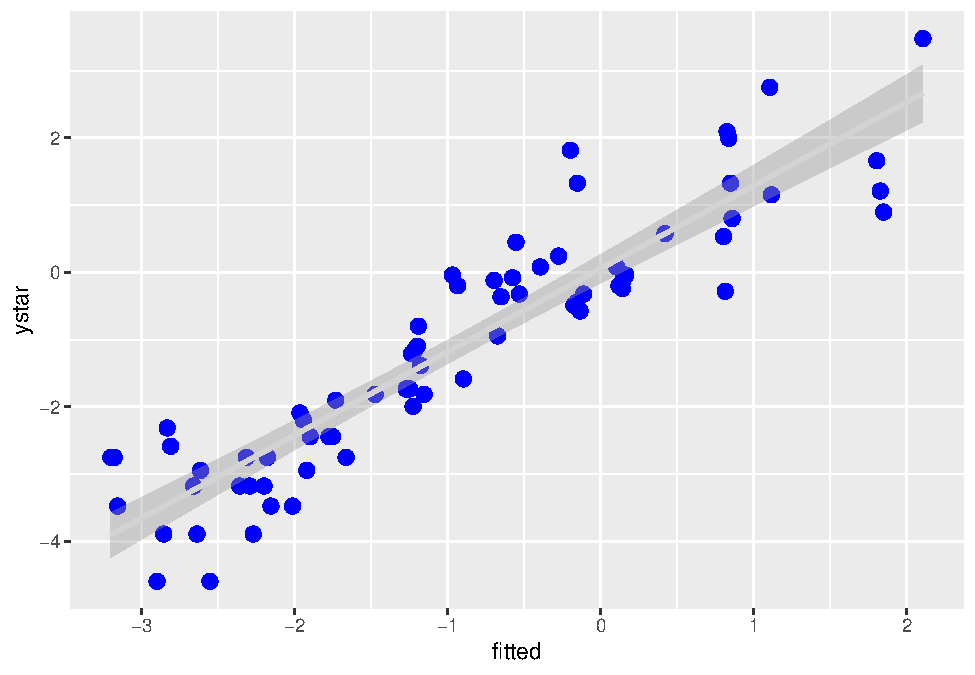
\includegraphics{01-ex4_files/figure-latex/obs-pred-plot-1.pdf}

\hypertarget{ex9_4}{%
\chapter{Exercise 9.4}\label{ex9_4}}

\hypertarget{load-packages-1}{%
\section{Load packages}\label{load-packages-1}}

Here is the R code to download the required packages for this exercise.

\begin{Shaded}
\begin{Highlighting}[]
\CommentTok{# install package manager 'pacman'}
\ControlFlowTok{if}\NormalTok{ (}\OperatorTok{!}\KeywordTok{require}\NormalTok{(pacman))\{}
  \KeywordTok{install.packages}\NormalTok{(}\StringTok{'pacman'}\NormalTok{)}
\NormalTok{\}}
\end{Highlighting}
\end{Shaded}

\begin{verbatim}
## Loading required package: pacman
\end{verbatim}

\begin{Shaded}
\begin{Highlighting}[]
\CommentTok{# load packages needed for this exercise}
\KeywordTok{library}\NormalTok{(pacman)}
\KeywordTok{p_load}\NormalTok{(tidyverse,}
\NormalTok{       lctools, }\CommentTok{# to calculate Moran's I}
\NormalTok{       spdep, }\CommentTok{# to calculate geary's c}
\NormalTok{       geoR, }\CommentTok{# to compute variogram}
\NormalTok{       gridExtra, }\CommentTok{# to stack plots}
\NormalTok{       gstat, automap, }\CommentTok{# packages for variogram model selection}
\NormalTok{       sp }\CommentTok{# need a function called `coordinates`}
\NormalTok{       )}
\end{Highlighting}
\end{Shaded}

\hypertarget{data}{%
\section{Data}\label{data}}

This is equivalent to data step in SAS. Here, the data is entered inside a function called \texttt{tibble}.

\begin{Shaded}
\begin{Highlighting}[]
\CommentTok{# Enter data}
\NormalTok{a <-}\StringTok{ }\KeywordTok{tibble}\NormalTok{(}\DataTypeTok{I =} \DecValTok{1}\OperatorTok{:}\DecValTok{16}\NormalTok{, }\DataTypeTok{YI =} \KeywordTok{c}\NormalTok{(}\DecValTok{41}\NormalTok{, }\DecValTok{60}\NormalTok{, }\DecValTok{81}\NormalTok{, }\DecValTok{22}\NormalTok{, }\DecValTok{8}\NormalTok{, }\DecValTok{20}\NormalTok{, }\DecValTok{28}\NormalTok{, }\DecValTok{2}\NormalTok{,}
                             \DecValTok{0}\NormalTok{, }\DecValTok{2}\NormalTok{, }\DecValTok{2}\NormalTok{, }\DecValTok{8}\NormalTok{, }\DecValTok{0}\NormalTok{, }\DecValTok{43}\NormalTok{, }\DecValTok{61}\NormalTok{, }\DecValTok{50}\NormalTok{)) }\OperatorTok\StringTok{ }
\StringTok{  }\CommentTok{# creat new variable East and North}
\StringTok{  }\KeywordTok{mutate}\NormalTok{(}\DataTypeTok{East =} \DecValTok{1}\NormalTok{,}
         \DataTypeTok{North =}\NormalTok{ I)}

\CommentTok{# print the data}
\NormalTok{a}
\end{Highlighting}
\end{Shaded}

\begin{verbatim}
## # A tibble: 16 x 4
##        I    YI  East North
##    <int> <dbl> <dbl> <int>
##  1     1    41     1     1
##  2     2    60     1     2
##  3     3    81     1     3
##  4     4    22     1     4
##  5     5     8     1     5
##  6     6    20     1     6
##  7     7    28     1     7
##  8     8     2     1     8
##  9     9     0     1     9
## 10    10     2     1    10
## 11    11     2     1    11
## 12    12     8     1    12
## 13    13     0     1    13
## 14    14    43     1    14
## 15    15    61     1    15
## 16    16    50     1    16
\end{verbatim}

\hypertarget{autocorrelation-statistics}{%
\section{Autocorrelation statistics}\label{autocorrelation-statistics}}

\begin{Shaded}
\begin{Highlighting}[]
\CommentTok{# visualize the data}
\KeywordTok{ggplot}\NormalTok{(}\DataTypeTok{data =}\NormalTok{ a) }\OperatorTok{+}
\StringTok{  }\KeywordTok{geom_point}\NormalTok{(}\DataTypeTok{mapping =} \KeywordTok{aes}\NormalTok{(}\DataTypeTok{x =}\NormalTok{ East, }\DataTypeTok{y =}\NormalTok{ North, }\DataTypeTok{size =}\NormalTok{ YI, }\DataTypeTok{color =}\NormalTok{ YI)) }\OperatorTok{+}
\StringTok{  }\KeywordTok{ggtitle}\NormalTok{(}\StringTok{"Spatial Distribution of YI Observation"}\NormalTok{) }\OperatorTok{+}
\StringTok{  }\KeywordTok{theme}\NormalTok{(}\DataTypeTok{plot.title =} \KeywordTok{element_text}\NormalTok{(}\DataTypeTok{hjust =} \FloatTok{0.5}\NormalTok{))}
\end{Highlighting}
\end{Shaded}

\includegraphics{02-ex9_4_files/figure-latex/autocorr-statistics-1.pdf}

\begin{Shaded}
\begin{Highlighting}[]
\CommentTok{# calculate Moran's I}
\NormalTok{Coords <-}\StringTok{ }\NormalTok{a }\OperatorTok\StringTok{ }
\StringTok{  }\NormalTok{dplyr}\OperatorTok{::}\KeywordTok{select}\NormalTok{(East, North)}

\NormalTok{mI <-}\StringTok{ }\KeywordTok{moransI}\NormalTok{(Coords, }\DataTypeTok{Bandwidth =} \DecValTok{1}\NormalTok{, a}\OperatorTok{$}\NormalTok{YI)}

\CommentTok{# print Moran's I table}
\NormalTok{moran.table <-}\StringTok{ }\KeywordTok{tribble}\NormalTok{(}
  \OperatorTok{~}\StringTok{`}\DataTypeTok{Moran's I}\StringTok{`}\NormalTok{, }\OperatorTok{~}\StringTok{`}\DataTypeTok{Expected I}\StringTok{`}\NormalTok{, }\OperatorTok{~}\StringTok{`}\DataTypeTok{Z randomization}\StringTok{`}\NormalTok{, }\OperatorTok{~}\StringTok{`}\DataTypeTok{P value randomization}\StringTok{`}\NormalTok{,}
  \CommentTok{#------------/--------------/-------------------/------------------------}
\NormalTok{  mI}\OperatorTok{$}\NormalTok{Morans.I, mI}\OperatorTok{$}\NormalTok{Expected.I,  mI}\OperatorTok{$}\NormalTok{z.randomization, mI}\OperatorTok{$}\NormalTok{p.value.randomization}
\NormalTok{  )}

\NormalTok{moran.table}
\end{Highlighting}
\end{Shaded}

\begin{verbatim}
## # A tibble: 1 x 4
##   `Moran's I` `Expected I` `Z randomization` `P value randomization`
##         <dbl>        <dbl>             <dbl>                   <dbl>
## 1       0.625      -0.0667              2.81                 0.00499
\end{verbatim}

\begin{Shaded}
\begin{Highlighting}[]
\CommentTok{# create Moran's I scatter plot}
\NormalTok{l.moran <-}\StringTok{ }\KeywordTok{l.moransI}\NormalTok{(Coords, }\DataTypeTok{Bandwidth =} \DecValTok{1}\NormalTok{, a}\OperatorTok{$}\NormalTok{YI)}
\end{Highlighting}
\end{Shaded}

\includegraphics{02-ex9_4_files/figure-latex/autocorr-statistics-2.pdf}

\begin{Shaded}
\begin{Highlighting}[]
\CommentTok{# calculate geary's c}
\NormalTok{Coords_num <-}\StringTok{ }\KeywordTok{coordinates}\NormalTok{(Coords)}

\CommentTok{# create an object of class 'nb' so that it can be used with function from packege `spdep`}
\NormalTok{Coords_nb <-}\StringTok{ }\KeywordTok{knn2nb}\NormalTok{(}\KeywordTok{knearneigh}\NormalTok{(Coords_num))}

\CommentTok{# create a 'listw' object for use in the function `geary.test`}
\NormalTok{coords_listw <-}\StringTok{ }\KeywordTok{nb2listw}\NormalTok{(Coords_nb)}

\NormalTok{gearyC <-}\StringTok{ }\KeywordTok{geary.test}\NormalTok{(a}\OperatorTok{$}\NormalTok{YI, coords_listw, }\DataTypeTok{alternative =} \StringTok{"two.sided"}\NormalTok{)}
\NormalTok{gearyC}
\end{Highlighting}
\end{Shaded}

\begin{verbatim}
## 
##  Geary C test under randomisation
## 
## data:  a$YI 
## weights: coords_listw 
## 
## Geary C statistic standard deviate = 2.5826, p-value = 0.009806
## alternative hypothesis: two.sided
## sample estimates:
## Geary C statistic       Expectation          Variance 
##        0.37085605        1.00000000        0.05934473
\end{verbatim}

\hypertarget{first-variogram}{%
\section{First variogram}\label{first-variogram}}

We will use the package \texttt{geoR} to construct empricial variogram, and then draw them using package \texttt{ggplot2}.

\begin{Shaded}
\begin{Highlighting}[]
\NormalTok{v1 <-}\StringTok{ }\KeywordTok{variog}\NormalTok{(}\DataTypeTok{coords =}\NormalTok{ Coords_num, }\DataTypeTok{data =}\NormalTok{ a}\OperatorTok{$}\NormalTok{YI, }\DataTypeTok{breaks =} \KeywordTok{seq}\NormalTok{(}\FloatTok{0.5}\NormalTok{, }\FloatTok{15.5}\NormalTok{),}
             \DataTypeTok{max.dist =} \DecValTok{11}\NormalTok{)}
\end{Highlighting}
\end{Shaded}

\begin{verbatim}
## variog: computing omnidirectional variogram
\end{verbatim}

\begin{Shaded}
\begin{Highlighting}[]
\CommentTok{# extract data from object v1 for plotting}
\NormalTok{v1_plot_data <-}\StringTok{ }\KeywordTok{cbind}\NormalTok{(v1}\OperatorTok{$}\NormalTok{u, v1}\OperatorTok{$}\NormalTok{v, v1}\OperatorTok{$}\NormalTok{n) }\OperatorTok\StringTok{ }
\StringTok{  }\KeywordTok{as.data.frame}\NormalTok{() }\OperatorTok\StringTok{ }
\StringTok{  }\NormalTok{dplyr}\OperatorTok{::}\KeywordTok{rename}\NormalTok{(}\DataTypeTok{Distance =}\NormalTok{ V1,}
                \DataTypeTok{Semivariance =}\NormalTok{ V2,}
                \DataTypeTok{Pair_count =}\NormalTok{ V3)}

\CommentTok{# in the table below, gamma is semivariance}
\NormalTok{v1_plot_data}
\end{Highlighting}
\end{Shaded}

\begin{verbatim}
##    Distance Semivariance Pair_count
## 1         1     258.8333         15
## 2         2     533.0000         14
## 3         3     576.6154         13
## 4         4     580.1667         12
## 5         5     754.0000         11
## 6         6     958.2000         10
## 7         7    1020.4444          9
## 8         8     966.7500          8
## 9         9    1006.2857          7
## 10       10    1244.6667          6
## 11       11     941.8000          5
\end{verbatim}

\begin{Shaded}
\begin{Highlighting}[]
\CommentTok{# plot variogram}
\NormalTok{v1_plot_vario <-}\StringTok{ }\KeywordTok{ggplot}\NormalTok{(}\DataTypeTok{data =}\NormalTok{ v1_plot_data) }\OperatorTok{+}
\StringTok{  }\KeywordTok{geom_point}\NormalTok{(}\DataTypeTok{mapping =} \KeywordTok{aes}\NormalTok{(}\DataTypeTok{x =}\NormalTok{ Distance, }\DataTypeTok{y =}\NormalTok{ Semivariance)) }\OperatorTok{+}
\StringTok{  }\KeywordTok{ggtitle}\NormalTok{(}\StringTok{"Empirical Semivariogram of YI"}\NormalTok{) }\OperatorTok{+}
\StringTok{  }\KeywordTok{theme}\NormalTok{(}\DataTypeTok{plot.title =} \KeywordTok{element_text}\NormalTok{(}\DataTypeTok{hjust =} \FloatTok{0.5}\NormalTok{))}

\CommentTok{# plot pair counts}
\NormalTok{v1_plot_pair_count <-}\StringTok{ }\KeywordTok{ggplot}\NormalTok{(}\DataTypeTok{data =}\NormalTok{ v1_plot_data) }\OperatorTok{+}
\StringTok{  }\KeywordTok{geom_col}\NormalTok{(}\DataTypeTok{mapping =} \KeywordTok{aes}\NormalTok{(}\DataTypeTok{x =}\NormalTok{ Distance, }\DataTypeTok{y =}\NormalTok{ Pair_count), }\DataTypeTok{width =} \FloatTok{0.01}\NormalTok{, }\DataTypeTok{color =} \StringTok{"blue"}\NormalTok{)}

\CommentTok{# stack two plots}
\KeywordTok{grid.arrange}\NormalTok{(v1_plot_vario, v1_plot_pair_count,}
             \DataTypeTok{ncol =} \DecValTok{1}\NormalTok{, }\DataTypeTok{heights =} \KeywordTok{c}\NormalTok{(}\DecValTok{3}\NormalTok{, }\DecValTok{1}\NormalTok{))}
\end{Highlighting}
\end{Shaded}

\includegraphics{02-ex9_4_files/figure-latex/first-variogram-model-1.pdf}

\hypertarget{second-variogram}{%
\section{Second variogram}\label{second-variogram}}

Plot robust and classical variogram together.

\begin{Shaded}
\begin{Highlighting}[]
\CommentTok{# fit robust variogram}
\NormalTok{v1_robust <-}\StringTok{ }\KeywordTok{variog}\NormalTok{(}\DataTypeTok{coords =}\NormalTok{ Coords_num, }\DataTypeTok{data =}\NormalTok{ a}\OperatorTok{$}\NormalTok{YI, }\DataTypeTok{breaks =} \KeywordTok{seq}\NormalTok{(}\FloatTok{0.5}\NormalTok{, }\FloatTok{15.5}\NormalTok{),}
             \DataTypeTok{max.dist =} \DecValTok{11}\NormalTok{, }\DataTypeTok{estimator.type =} \StringTok{"modulus"}\NormalTok{)}
\end{Highlighting}
\end{Shaded}

\begin{verbatim}
## variog: computing omnidirectional variogram
\end{verbatim}

\begin{Shaded}
\begin{Highlighting}[]
\CommentTok{# extract the data}
\NormalTok{v1_robust_data <-}\StringTok{ }\KeywordTok{cbind}\NormalTok{(v1_robust}\OperatorTok{$}\NormalTok{u, v1_robust}\OperatorTok{$}\NormalTok{v, v1_robust}\OperatorTok{$}\NormalTok{n) }\OperatorTok\StringTok{ }
\StringTok{  }\KeywordTok{as.data.frame}\NormalTok{() }\OperatorTok\StringTok{ }
\StringTok{  }\NormalTok{dplyr}\OperatorTok{::}\KeywordTok{rename}\NormalTok{(}\DataTypeTok{Distance =}\NormalTok{ V1,}
                \DataTypeTok{Semivariance =}\NormalTok{ V2,}
                \DataTypeTok{Pair_count =}\NormalTok{ V3)}

\CommentTok{# plot robust variogram}
\NormalTok{v1_robust_vario <-}\StringTok{ }\KeywordTok{ggplot}\NormalTok{(}\DataTypeTok{data =}\NormalTok{ v1_robust_data) }\OperatorTok{+}
\StringTok{  }\KeywordTok{geom_point}\NormalTok{(}\DataTypeTok{mapping =} \KeywordTok{aes}\NormalTok{(}\DataTypeTok{x =}\NormalTok{ Distance, }\DataTypeTok{y =}\NormalTok{ Semivariance)) }\OperatorTok{+}
\StringTok{  }\KeywordTok{ggtitle}\NormalTok{(}\StringTok{"Empirical Semivariogram of YI - Robust estimation"}\NormalTok{) }\OperatorTok{+}
\StringTok{  }\KeywordTok{theme}\NormalTok{(}\DataTypeTok{plot.title =} \KeywordTok{element_text}\NormalTok{(}\DataTypeTok{hjust =} \FloatTok{0.5}\NormalTok{))}

\NormalTok{v1_robust_vario}
\end{Highlighting}
\end{Shaded}

\includegraphics{02-ex9_4_files/figure-latex/second-variogram-model-1.pdf}

\begin{Shaded}
\begin{Highlighting}[]
\CommentTok{# combine robust and classical variogram  }
\NormalTok{var_comb <-}\StringTok{ }\NormalTok{v1_robust_data }\OperatorTok\StringTok{ }
\StringTok{  }
\StringTok{  }\CommentTok{# combine robust and classical variogram datasets}
\StringTok{  }\NormalTok{dplyr}\OperatorTok{::}\KeywordTok{rename}\NormalTok{(}\DataTypeTok{Semivariance_robust =}\NormalTok{ Semivariance) }\OperatorTok\StringTok{ }
\StringTok{  }\KeywordTok{bind_cols}\NormalTok{(dplyr}\OperatorTok{::}\KeywordTok{select}\NormalTok{(v1_plot_data, Semivariance)) }\OperatorTok\StringTok{ }
\StringTok{  }\KeywordTok{gather}\NormalTok{(}\DataTypeTok{key =} \StringTok{"Semivariance_type"}\NormalTok{, }\DataTypeTok{value =} \StringTok{"Semivariance"}\NormalTok{, }\OperatorTok{-}\KeywordTok{c}\NormalTok{(Distance, Pair_count)) }\OperatorTok\StringTok{ }
\StringTok{  }
\StringTok{  }\CommentTok{# plot}
\StringTok{  }\KeywordTok{ggplot}\NormalTok{() }\OperatorTok{+}
\StringTok{  }\KeywordTok{geom_point}\NormalTok{(}\DataTypeTok{mapping =} \KeywordTok{aes}\NormalTok{(}\DataTypeTok{x =}\NormalTok{ Distance, }\DataTypeTok{y =}\NormalTok{ Semivariance, }\DataTypeTok{color =}\NormalTok{ Semivariance_type)) }\OperatorTok{+}
\StringTok{  }\KeywordTok{ggtitle}\NormalTok{(}\StringTok{"Empirical Semivariogram for YI"}\NormalTok{) }\OperatorTok{+}
\StringTok{  }\KeywordTok{theme}\NormalTok{(}\DataTypeTok{plot.title =} \KeywordTok{element_text}\NormalTok{(}\DataTypeTok{hjust =} \FloatTok{0.5}\NormalTok{))}

\NormalTok{var_comb}
\end{Highlighting}
\end{Shaded}

\includegraphics{02-ex9_4_files/figure-latex/second-variogram-model-2.pdf}

\hypertarget{variogram-model-selection}{%
\section{Variogram model selection}\label{variogram-model-selection}}

We will use the package \texttt{gstat} and \texttt{automap} for variogram model selection

\begin{Shaded}
\begin{Highlighting}[]
\CommentTok{# specify coordinates in the dataset}
\KeywordTok{coordinates}\NormalTok{(a) =}\StringTok{ }\ErrorTok{~}\NormalTok{East}\OperatorTok{+}\NormalTok{North}

\CommentTok{# select the best model out of exponential, spherical, and gaussian  }
\KeywordTok{autofitVariogram}\NormalTok{(YI }\OperatorTok{~}\StringTok{ }\NormalTok{East }\OperatorTok{+}\StringTok{ }\NormalTok{North, a, }\DataTypeTok{model =} \KeywordTok{c}\NormalTok{(}\StringTok{"Sph"}\NormalTok{, }\StringTok{"Exp"}\NormalTok{, }\StringTok{"Gau"}\NormalTok{))}
\end{Highlighting}
\end{Shaded}

\begin{verbatim}
## $exp_var
##   np dist    gamma dir.hor dir.ver   id
## 1 15    1 258.8333       0       0 var1
## 2 14    2 533.0000       0       0 var1
## 3 13    3 576.6154       0       0 var1
## 4 12    4 580.1667       0       0 var1
## 5 11    5 754.0000       0       0 var1
## 
## $var_model
##   model    psill    range
## 1   Nug   0.0000 0.000000
## 2   Exp 854.3133 2.575499
## 
## $sserr
## [1] 28783.32
## 
## attr(,"class")
## [1] "autofitVariogram" "list"
\end{verbatim}

\begin{Shaded}
\begin{Highlighting}[]
\CommentTok{# fit empirical variogram}
\NormalTok{v_emp <-}\StringTok{ }\KeywordTok{variogram}\NormalTok{(YI }\OperatorTok{~}\StringTok{ }\NormalTok{East }\OperatorTok{+}\StringTok{ }\NormalTok{North, }\DataTypeTok{data =}\NormalTok{ a, }\DataTypeTok{cutoff =} \DecValTok{11}\NormalTok{)}
\NormalTok{v_emp}
\end{Highlighting}
\end{Shaded}

\begin{verbatim}
##    np dist     gamma dir.hor dir.ver   id
## 1  15    1  258.8333       0       0 var1
## 2  14    2  533.0000       0       0 var1
## 3  13    3  576.6154       0       0 var1
## 4  12    4  580.1667       0       0 var1
## 5  11    5  754.0000       0       0 var1
## 6  10    6  958.2000       0       0 var1
## 7   9    7 1020.4444       0       0 var1
## 8   8    8  966.7500       0       0 var1
## 9   7    9 1006.2857       0       0 var1
## 10  6   10 1244.6667       0       0 var1
## 11  5   11  941.8000       0       0 var1
\end{verbatim}

\begin{Shaded}
\begin{Highlighting}[]
\KeywordTok{plot}\NormalTok{(v_emp)}
\end{Highlighting}
\end{Shaded}

\includegraphics{02-ex9_4_files/figure-latex/model-selection-1.pdf}

\begin{Shaded}
\begin{Highlighting}[]
\CommentTok{# fit exponential variogram}
\NormalTok{v_exp <-}\StringTok{ }\KeywordTok{fit.variogram}\NormalTok{(v_emp, }\KeywordTok{vgm}\NormalTok{(}\StringTok{"Exp"}\NormalTok{))}
\NormalTok{v_exp}
\end{Highlighting}
\end{Shaded}

\begin{verbatim}
##   model    psill   range
## 1   Nug    0.000 0.00000
## 2   Exp 1062.461 3.47171
\end{verbatim}

\begin{Shaded}
\begin{Highlighting}[]
\CommentTok{# fit spherical and gaussian}
\NormalTok{v_sph <-}\StringTok{ }\KeywordTok{fit.variogram}\NormalTok{(v_emp, }\KeywordTok{vgm}\NormalTok{(}\StringTok{"Sph"}\NormalTok{))}
\NormalTok{v_gau <-}\StringTok{ }\KeywordTok{fit.variogram}\NormalTok{(v_emp, }\KeywordTok{vgm}\NormalTok{(}\StringTok{"Gau"}\NormalTok{))}

\CommentTok{# extract plotting data from fitted variograms}
\NormalTok{v_exp_line <-}\StringTok{ }\KeywordTok{variogramLine}\NormalTok{(v_exp, }\DataTypeTok{maxdist =} \DecValTok{11}\NormalTok{)}
\NormalTok{v_sph_line <-}\StringTok{ }\KeywordTok{variogramLine}\NormalTok{(v_sph, }\DataTypeTok{maxdist =} \DecValTok{11}\NormalTok{)}
\NormalTok{v_gau_line <-}\StringTok{ }\KeywordTok{variogramLine}\NormalTok{(v_gau, }\DataTypeTok{maxdist =} \DecValTok{11}\NormalTok{)}

\CommentTok{# plot emprical and fitted variograms together  }
\CommentTok{# specify color for legends}
\NormalTok{legend_color <-}\StringTok{ }\KeywordTok{c}\NormalTok{(}\StringTok{"Empirical"}\NormalTok{ =}\StringTok{ "blue"}\NormalTok{, }\StringTok{"Exponential"}\NormalTok{ =}\StringTok{ "blue"}\NormalTok{,}
                  \StringTok{"Spherical"}\NormalTok{ =}\StringTok{ "orange"}\NormalTok{, }\StringTok{"Gaussian"}\NormalTok{ =}\StringTok{ "green"}\NormalTok{)}
\KeywordTok{ggplot}\NormalTok{(}\DataTypeTok{data =}\NormalTok{ v_emp) }\OperatorTok{+}
\StringTok{  }\KeywordTok{geom_point}\NormalTok{(}\DataTypeTok{mapping =} \KeywordTok{aes}\NormalTok{(}\DataTypeTok{x =}\NormalTok{ dist, }\DataTypeTok{y =}\NormalTok{ gamma, }\DataTypeTok{fill =} \StringTok{"Empirical"}\NormalTok{), }\DataTypeTok{color =} \StringTok{"blue"}\NormalTok{) }\OperatorTok{+}
\StringTok{  }\KeywordTok{geom_line}\NormalTok{(}\DataTypeTok{data =}\NormalTok{ v_exp_line, }\DataTypeTok{mapping =} \KeywordTok{aes}\NormalTok{(}\DataTypeTok{x =}\NormalTok{ dist, }\DataTypeTok{y =}\NormalTok{ gamma, }\DataTypeTok{color =} \StringTok{"Exponential"}\NormalTok{)) }\OperatorTok{+}
\StringTok{  }\KeywordTok{geom_line}\NormalTok{(}\DataTypeTok{data =}\NormalTok{ v_sph_line, }\DataTypeTok{mapping =} \KeywordTok{aes}\NormalTok{(}\DataTypeTok{x =}\NormalTok{ dist, }\DataTypeTok{y =}\NormalTok{ gamma, }\DataTypeTok{color =} \StringTok{"Spherical"}\NormalTok{)) }\OperatorTok{+}
\StringTok{  }\KeywordTok{geom_line}\NormalTok{(}\DataTypeTok{data =}\NormalTok{ v_gau_line, }\DataTypeTok{mapping =} \KeywordTok{aes}\NormalTok{(}\DataTypeTok{x =}\NormalTok{ dist, }\DataTypeTok{y =}\NormalTok{ gamma, }\DataTypeTok{color =} \StringTok{"Gaussian"}\NormalTok{)) }\OperatorTok{+}
\StringTok{  }\KeywordTok{scale_color_manual}\NormalTok{(}\DataTypeTok{name =} \StringTok{""}\NormalTok{, }\DataTypeTok{values =}\NormalTok{ legend_color) }\OperatorTok{+}
\StringTok{  }\KeywordTok{scale_fill_manual}\NormalTok{(}\DataTypeTok{name =} \StringTok{""}\NormalTok{, }\DataTypeTok{values =}\NormalTok{ legend_color) }\OperatorTok{+}
\StringTok{  }\KeywordTok{labs}\NormalTok{(}\DataTypeTok{x =} \StringTok{"Distance"}\NormalTok{,}
       \DataTypeTok{y =} \StringTok{"Semivariance"}\NormalTok{)}
\end{Highlighting}
\end{Shaded}

\includegraphics{02-ex9_4_files/figure-latex/model-selection-2.pdf}

\hypertarget{ex9_5}{%
\chapter{Exercise 9.5}\label{ex9_5}}

\hypertarget{load-packages-2}{%
\section{Load packages}\label{load-packages-2}}

Here is the R code to download the required packages for this exercise.

\begin{Shaded}
\begin{Highlighting}[]
\CommentTok{# install package manager 'pacman'}
\ControlFlowTok{if}\NormalTok{ (}\OperatorTok{!}\KeywordTok{require}\NormalTok{(pacman))\{}
  \KeywordTok{install.packages}\NormalTok{(}\StringTok{'pacman'}\NormalTok{)}
\NormalTok{\}}
\end{Highlighting}
\end{Shaded}

\begin{verbatim}
## Loading required package: pacman
\end{verbatim}

\begin{Shaded}
\begin{Highlighting}[]
\CommentTok{# load packages needed for this exercise}
\KeywordTok{library}\NormalTok{(pacman)}
\KeywordTok{p_load}\NormalTok{(tidyverse,}
\NormalTok{       lctools, }\CommentTok{# to calculate Moran's I}
\NormalTok{       spdep, }\CommentTok{# to calculate geary's c}
\NormalTok{       geoR, }\CommentTok{# to compute variogram}
\NormalTok{       gridExtra, }\CommentTok{# to stack plots}
\NormalTok{       gstat, automap, }\CommentTok{# packages for variogram model selection}
\NormalTok{       sp }\CommentTok{# need a function called `coordinates`}
\NormalTok{       )}
\end{Highlighting}
\end{Shaded}

\hypertarget{data-1}{%
\section{Data}\label{data-1}}

This is equivalent to data step in SAS. Here, the data is imported from a file \texttt{data.csv} using the function \texttt{read\_csv}. This function will download the file directly from \href{https://raw.githubusercontent.com/luckymehra/epidem-exercises/master/data/ex9_5.csv}{here}.

\begin{Shaded}
\begin{Highlighting}[]
\CommentTok{# Import data}
\NormalTok{a <-}\StringTok{ }\KeywordTok{read_csv}\NormalTok{(}\StringTok{"https://raw.githubusercontent.com/luckymehra/epidem-exercises/master/data/ex9_5.csv"}\NormalTok{)}
\end{Highlighting}
\end{Shaded}

\begin{verbatim}
## Parsed with column specification:
## cols(
##   COL = col_double(),
##   ROW = col_double(),
##   YI = col_double()
## )
\end{verbatim}

\begin{Shaded}
\begin{Highlighting}[]
\CommentTok{# print the data}
\NormalTok{a}
\end{Highlighting}
\end{Shaded}

\begin{verbatim}
## # A tibble: 144 x 3
##      COL   ROW    YI
##    <dbl> <dbl> <dbl>
##  1     1     1     2
##  2     2     1     2
##  3     3     1     0
##  4     4     1     3
##  5     5     1     1
##  6     6     1     1
##  7     7     1     1
##  8     8     1     5
##  9     9     1    22
## 10    10     1    13
## # ... with 134 more rows
\end{verbatim}

\hypertarget{autocorrelation-statistics-1}{%
\section{Autocorrelation statistics}\label{autocorrelation-statistics-1}}

\begin{Shaded}
\begin{Highlighting}[]
\CommentTok{# visualize the data}
\KeywordTok{ggplot}\NormalTok{(}\DataTypeTok{data =}\NormalTok{ a) }\OperatorTok{+}
\StringTok{  }\KeywordTok{geom_point}\NormalTok{(}\DataTypeTok{mapping =} \KeywordTok{aes}\NormalTok{(}\DataTypeTok{x =}\NormalTok{ COL, }\DataTypeTok{y =}\NormalTok{ ROW, }\DataTypeTok{size =}\NormalTok{ YI, }\DataTypeTok{color =}\NormalTok{ YI)) }\OperatorTok{+}
\StringTok{  }\KeywordTok{ggtitle}\NormalTok{(}\StringTok{"Spatial Distribution of YI Observation"}\NormalTok{) }\OperatorTok{+}
\StringTok{  }\KeywordTok{theme}\NormalTok{(}\DataTypeTok{plot.title =} \KeywordTok{element_text}\NormalTok{(}\DataTypeTok{hjust =} \FloatTok{0.5}\NormalTok{))}
\end{Highlighting}
\end{Shaded}

\includegraphics{03-ex9_5_files/figure-latex/autocorr-statistics-1.pdf}

\begin{Shaded}
\begin{Highlighting}[]
\CommentTok{# calculate Moran's I}
\NormalTok{Coords <-}\StringTok{ }\NormalTok{a }\OperatorTok\StringTok{ }
\StringTok{  }\NormalTok{dplyr}\OperatorTok{::}\KeywordTok{select}\NormalTok{(COL, ROW)}

\NormalTok{mI <-}\StringTok{ }\KeywordTok{moransI}\NormalTok{(Coords, }\DataTypeTok{Bandwidth =} \DecValTok{1}\NormalTok{, a}\OperatorTok{$}\NormalTok{YI)}

\CommentTok{# print Moran's I table}
\NormalTok{moran.table <-}\StringTok{ }\KeywordTok{tribble}\NormalTok{(}
  \OperatorTok{~}\StringTok{`}\DataTypeTok{Moran's I}\StringTok{`}\NormalTok{, }\OperatorTok{~}\StringTok{`}\DataTypeTok{Expected I}\StringTok{`}\NormalTok{, }\OperatorTok{~}\StringTok{`}\DataTypeTok{Z randomization}\StringTok{`}\NormalTok{, }\OperatorTok{~}\StringTok{`}\DataTypeTok{P value randomization}\StringTok{`}\NormalTok{,}
  \CommentTok{#------------/--------------/-------------------/------------------------}
\NormalTok{  mI}\OperatorTok{$}\NormalTok{Morans.I, mI}\OperatorTok{$}\NormalTok{Expected.I,  mI}\OperatorTok{$}\NormalTok{z.randomization, mI}\OperatorTok{$}\NormalTok{p.value.randomization}
\NormalTok{  )}

\NormalTok{moran.table}
\end{Highlighting}
\end{Shaded}

\begin{verbatim}
## # A tibble: 1 x 4
##   `Moran's I` `Expected I` `Z randomization` `P value randomization`
##         <dbl>        <dbl>             <dbl>                   <dbl>
## 1       0.782     -0.00699              13.0                1.28e-38
\end{verbatim}

\begin{Shaded}
\begin{Highlighting}[]
\CommentTok{# create Moran's I scatter plot}
\NormalTok{l.moran <-}\StringTok{ }\KeywordTok{l.moransI}\NormalTok{(Coords, }\DataTypeTok{Bandwidth =} \DecValTok{1}\NormalTok{, a}\OperatorTok{$}\NormalTok{YI)}
\end{Highlighting}
\end{Shaded}

\includegraphics{03-ex9_5_files/figure-latex/autocorr-statistics-2.pdf}

\begin{Shaded}
\begin{Highlighting}[]
\CommentTok{# calculate geary's c}
\NormalTok{Coords_num <-}\StringTok{ }\KeywordTok{coordinates}\NormalTok{(Coords)}

\CommentTok{# create an object of class 'nb' so that it can be used with function from packege `spdep`}
\NormalTok{Coords_nb <-}\StringTok{ }\KeywordTok{knn2nb}\NormalTok{(}\KeywordTok{knearneigh}\NormalTok{(Coords_num))}

\CommentTok{# create a 'listw' object for use in the function `geary.test`}
\NormalTok{coords_listw <-}\StringTok{ }\KeywordTok{nb2listw}\NormalTok{(Coords_nb)}

\NormalTok{gearyC <-}\StringTok{ }\KeywordTok{geary.test}\NormalTok{(a}\OperatorTok{$}\NormalTok{YI, coords_listw, }\DataTypeTok{alternative =} \StringTok{"two.sided"}\NormalTok{)}
\NormalTok{gearyC}
\end{Highlighting}
\end{Shaded}

\begin{verbatim}
## 
##  Geary C test under randomisation
## 
## data:  a$YI 
## weights: coords_listw 
## 
## Geary C statistic standard deviate = 8.8657, p-value < 2.2e-16
## alternative hypothesis: two.sided
## sample estimates:
## Geary C statistic       Expectation          Variance 
##       0.235058006       1.000000000       0.007444457
\end{verbatim}

\hypertarget{first-variogram-1}{%
\section{First variogram}\label{first-variogram-1}}

We will use the package \texttt{geoR} to construct empricial variogram, and then draw them using package \texttt{ggplot2}.

\begin{Shaded}
\begin{Highlighting}[]
\NormalTok{v1 <-}\StringTok{ }\KeywordTok{variog}\NormalTok{(}\DataTypeTok{coords =}\NormalTok{ Coords_num, }\DataTypeTok{data =}\NormalTok{ a}\OperatorTok{$}\NormalTok{YI, }\DataTypeTok{breaks =} \KeywordTok{seq}\NormalTok{(}\FloatTok{0.5}\NormalTok{, }\FloatTok{15.5}\NormalTok{),}
             \DataTypeTok{max.dist =} \DecValTok{12}\NormalTok{)}
\end{Highlighting}
\end{Shaded}

\begin{verbatim}
## variog: computing omnidirectional variogram
\end{verbatim}

\begin{Shaded}
\begin{Highlighting}[]
\CommentTok{# extract data from object v1 for plotting}
\NormalTok{v1_plot_data <-}\StringTok{ }\KeywordTok{cbind}\NormalTok{(v1}\OperatorTok{$}\NormalTok{u, v1}\OperatorTok{$}\NormalTok{v, v1}\OperatorTok{$}\NormalTok{n) }\OperatorTok\StringTok{ }
\StringTok{  }\KeywordTok{as.data.frame}\NormalTok{() }\OperatorTok\StringTok{ }
\StringTok{  }\NormalTok{dplyr}\OperatorTok{::}\KeywordTok{rename}\NormalTok{(}\DataTypeTok{Distance =}\NormalTok{ V1,}
                \DataTypeTok{Semivariance =}\NormalTok{ V2,}
                \DataTypeTok{Pair_count =}\NormalTok{ V3)}

\CommentTok{# in the table below, gamma is semivariance}
\NormalTok{v1_plot_data}
\end{Highlighting}
\end{Shaded}

\begin{verbatim}
##    Distance Semivariance Pair_count
## 1         1     311.7154        506
## 2         2     636.2074        680
## 3         3     818.7044        812
## 4         4     901.3218       1386
## 5         5     910.2773       1044
## 6         6     942.3219       1252
## 7         7     998.2290       1046
## 8         8    1131.2105       1012
## 9         9    1261.6817       1076
## 10       10    1219.6067        614
## 11       11    1166.5541        508
## 12       12     910.6250         80
\end{verbatim}

\begin{Shaded}
\begin{Highlighting}[]
\CommentTok{# plot variogram}
\NormalTok{v1_plot_vario <-}\StringTok{ }\KeywordTok{ggplot}\NormalTok{(}\DataTypeTok{data =}\NormalTok{ v1_plot_data) }\OperatorTok{+}
\StringTok{  }\KeywordTok{geom_point}\NormalTok{(}\DataTypeTok{mapping =} \KeywordTok{aes}\NormalTok{(}\DataTypeTok{x =}\NormalTok{ Distance, }\DataTypeTok{y =}\NormalTok{ Semivariance)) }\OperatorTok{+}
\StringTok{  }\KeywordTok{ggtitle}\NormalTok{(}\StringTok{"Empirical Semivariogram of YI"}\NormalTok{) }\OperatorTok{+}
\StringTok{  }\KeywordTok{theme}\NormalTok{(}\DataTypeTok{plot.title =} \KeywordTok{element_text}\NormalTok{(}\DataTypeTok{hjust =} \FloatTok{0.5}\NormalTok{))}

\CommentTok{# plot pair counts}
\NormalTok{v1_plot_pair_count <-}\StringTok{ }\KeywordTok{ggplot}\NormalTok{(}\DataTypeTok{data =}\NormalTok{ v1_plot_data) }\OperatorTok{+}
\StringTok{  }\KeywordTok{geom_col}\NormalTok{(}\DataTypeTok{mapping =} \KeywordTok{aes}\NormalTok{(}\DataTypeTok{x =}\NormalTok{ Distance, }\DataTypeTok{y =}\NormalTok{ Pair_count), }\DataTypeTok{width =} \FloatTok{0.01}\NormalTok{, }\DataTypeTok{color =} \StringTok{"blue"}\NormalTok{)}

\CommentTok{# stack two plots}
\KeywordTok{grid.arrange}\NormalTok{(v1_plot_vario, v1_plot_pair_count,}
             \DataTypeTok{ncol =} \DecValTok{1}\NormalTok{, }\DataTypeTok{heights =} \KeywordTok{c}\NormalTok{(}\DecValTok{3}\NormalTok{, }\DecValTok{1}\NormalTok{))}
\end{Highlighting}
\end{Shaded}

\includegraphics{03-ex9_5_files/figure-latex/first-variogram-model-1.pdf}

\hypertarget{second-variogram-1}{%
\section{Second variogram}\label{second-variogram-1}}

Plot robust and classical variogram together.

\begin{Shaded}
\begin{Highlighting}[]
\CommentTok{# fit robust variogram}
\NormalTok{v1_robust <-}\StringTok{ }\KeywordTok{variog}\NormalTok{(}\DataTypeTok{coords =}\NormalTok{ Coords_num, }\DataTypeTok{data =}\NormalTok{ a}\OperatorTok{$}\NormalTok{YI, }\DataTypeTok{breaks =} \KeywordTok{seq}\NormalTok{(}\FloatTok{0.5}\NormalTok{, }\FloatTok{15.5}\NormalTok{),}
             \DataTypeTok{max.dist =} \DecValTok{12}\NormalTok{, }\DataTypeTok{estimator.type =} \StringTok{"modulus"}\NormalTok{)}
\end{Highlighting}
\end{Shaded}

\begin{verbatim}
## variog: computing omnidirectional variogram
\end{verbatim}

\begin{Shaded}
\begin{Highlighting}[]
\CommentTok{# extract the data}
\NormalTok{v1_robust_data <-}\StringTok{ }\KeywordTok{cbind}\NormalTok{(v1_robust}\OperatorTok{$}\NormalTok{u, v1_robust}\OperatorTok{$}\NormalTok{v, v1_robust}\OperatorTok{$}\NormalTok{n) }\OperatorTok\StringTok{ }
\StringTok{  }\KeywordTok{as.data.frame}\NormalTok{() }\OperatorTok\StringTok{ }
\StringTok{  }\NormalTok{dplyr}\OperatorTok{::}\KeywordTok{rename}\NormalTok{(}\DataTypeTok{Distance =}\NormalTok{ V1,}
                \DataTypeTok{Semivariance =}\NormalTok{ V2,}
                \DataTypeTok{Pair_count =}\NormalTok{ V3)}

\CommentTok{# plot robust variogram}
\NormalTok{v1_robust_vario <-}\StringTok{ }\KeywordTok{ggplot}\NormalTok{(}\DataTypeTok{data =}\NormalTok{ v1_robust_data) }\OperatorTok{+}
\StringTok{  }\KeywordTok{geom_point}\NormalTok{(}\DataTypeTok{mapping =} \KeywordTok{aes}\NormalTok{(}\DataTypeTok{x =}\NormalTok{ Distance, }\DataTypeTok{y =}\NormalTok{ Semivariance)) }\OperatorTok{+}
\StringTok{  }\KeywordTok{ggtitle}\NormalTok{(}\StringTok{"Empirical Semivariogram of YI - Robust estimation"}\NormalTok{) }\OperatorTok{+}
\StringTok{  }\KeywordTok{theme}\NormalTok{(}\DataTypeTok{plot.title =} \KeywordTok{element_text}\NormalTok{(}\DataTypeTok{hjust =} \FloatTok{0.5}\NormalTok{))}

\NormalTok{v1_robust_vario}
\end{Highlighting}
\end{Shaded}

\includegraphics{03-ex9_5_files/figure-latex/second-variogram-model-1.pdf}

\begin{Shaded}
\begin{Highlighting}[]
\CommentTok{# combine robust and classical variogram  }
\NormalTok{var_comb <-}\StringTok{ }\NormalTok{v1_robust_data }\OperatorTok\StringTok{ }
\StringTok{  }
\StringTok{  }\CommentTok{# combine robust and classical variogram datasets}
\StringTok{  }\NormalTok{dplyr}\OperatorTok{::}\KeywordTok{rename}\NormalTok{(}\DataTypeTok{Semivariance_robust =}\NormalTok{ Semivariance) }\OperatorTok\StringTok{ }
\StringTok{  }\KeywordTok{bind_cols}\NormalTok{(dplyr}\OperatorTok{::}\KeywordTok{select}\NormalTok{(v1_plot_data, Semivariance)) }\OperatorTok\StringTok{ }
\StringTok{  }\KeywordTok{gather}\NormalTok{(}\DataTypeTok{key =} \StringTok{"Semivariance_type"}\NormalTok{, }\DataTypeTok{value =} \StringTok{"Semivariance"}\NormalTok{, }\OperatorTok{-}\KeywordTok{c}\NormalTok{(Distance, Pair_count)) }\OperatorTok\StringTok{ }
\StringTok{  }
\StringTok{  }\CommentTok{# plot}
\StringTok{  }\KeywordTok{ggplot}\NormalTok{() }\OperatorTok{+}
\StringTok{  }\KeywordTok{geom_point}\NormalTok{(}\DataTypeTok{mapping =} \KeywordTok{aes}\NormalTok{(}\DataTypeTok{x =}\NormalTok{ Distance, }\DataTypeTok{y =}\NormalTok{ Semivariance, }\DataTypeTok{color =}\NormalTok{ Semivariance_type)) }\OperatorTok{+}
\StringTok{  }\KeywordTok{ggtitle}\NormalTok{(}\StringTok{"Empirical Semivariogram for YI"}\NormalTok{) }\OperatorTok{+}
\StringTok{  }\KeywordTok{theme}\NormalTok{(}\DataTypeTok{plot.title =} \KeywordTok{element_text}\NormalTok{(}\DataTypeTok{hjust =} \FloatTok{0.5}\NormalTok{))}

\NormalTok{var_comb}
\end{Highlighting}
\end{Shaded}

\includegraphics{03-ex9_5_files/figure-latex/second-variogram-model-2.pdf}

\hypertarget{variogram-model-selection-1}{%
\section{Variogram model selection}\label{variogram-model-selection-1}}

We will use the package \texttt{gstat} and \texttt{automap} for variogram model selection

\begin{Shaded}
\begin{Highlighting}[]
\CommentTok{# specify coordinates in the dataset}
\KeywordTok{coordinates}\NormalTok{(a) =}\StringTok{ }\ErrorTok{~}\NormalTok{COL}\OperatorTok{+}\NormalTok{ROW}

\CommentTok{# select the best model out of exponential, spherical, and gaussian  }
\KeywordTok{autofitVariogram}\NormalTok{(YI }\OperatorTok{~}\StringTok{ }\NormalTok{COL }\OperatorTok{+}\StringTok{ }\NormalTok{ROW, a, }\DataTypeTok{model =} \KeywordTok{c}\NormalTok{(}\StringTok{"Sph"}\NormalTok{, }\StringTok{"Exp"}\NormalTok{, }\StringTok{"Gau"}\NormalTok{), }\DataTypeTok{cutoff =} \DecValTok{12}\NormalTok{)}
\end{Highlighting}
\end{Shaded}

\begin{verbatim}
## $exp_var
##     np     dist    gamma dir.hor dir.ver   id
## 1  264 1.000000 233.2400       0       0 var1
## 2  242 1.414214 388.5222       0       0 var1
## 3  680 2.152750 612.6985       0       0 var1
## 4  812 3.036881 756.8971       0       0 var1
## 5 1066 3.944315 783.1461       0       0 var1
## 6 1364 4.977586 742.6252       0       0 var1
## 
## $var_model
##   model    psill    range
## 1   Nug   0.0000 0.000000
## 2   Sph 782.9935 4.019145
## 
## $sserr
## [1] 1247749
## 
## attr(,"class")
## [1] "autofitVariogram" "list"
\end{verbatim}

\begin{Shaded}
\begin{Highlighting}[]
\CommentTok{# fit empirical variogram}
\NormalTok{v_emp <-}\StringTok{ }\KeywordTok{variogram}\NormalTok{(YI }\OperatorTok{~}\StringTok{ }\NormalTok{COL }\OperatorTok{+}\StringTok{ }\NormalTok{ROW, }\DataTypeTok{data =}\NormalTok{ a, }\DataTypeTok{cutoff =} \DecValTok{12}\NormalTok{)}
\NormalTok{v_emp}
\end{Highlighting}
\end{Shaded}

\begin{verbatim}
##      np      dist    gamma dir.hor dir.ver   id
## 1   506  1.198102 307.5054       0       0 var1
## 2   680  2.152750 612.6985       0       0 var1
## 3   812  3.036881 756.8971       0       0 var1
## 4   552  3.742751 784.3027       0       0 var1
## 5   834  4.280245 782.1560       0       0 var1
## 6  1044  5.132514 730.3844       0       0 var1
## 7  1028  6.012860 693.9058       0       0 var1
## 8   878  6.801676 675.9157       0       0 var1
## 9   836  7.525735 703.4337       0       0 var1
## 10  852  8.302717 728.0099       0       0 var1
## 11  792  9.194510 712.3311       0       0 var1
## 12  542 10.047104 621.2100       0       0 var1
## 13  452 10.826377 554.3985       0       0 var1
## 14  208 11.494850 599.2237       0       0 var1
\end{verbatim}

\begin{Shaded}
\begin{Highlighting}[]
\KeywordTok{plot}\NormalTok{(v_emp)}
\end{Highlighting}
\end{Shaded}

\includegraphics{03-ex9_5_files/figure-latex/model-selection-1.pdf}

\begin{Shaded}
\begin{Highlighting}[]
\CommentTok{# fit exponential variogram}
\NormalTok{v_exp <-}\StringTok{ }\KeywordTok{fit.variogram}\NormalTok{(v_emp, }\KeywordTok{vgm}\NormalTok{(}\StringTok{"Exp"}\NormalTok{))}

\CommentTok{# fit spherical and gaussian}
\NormalTok{v_sph <-}\StringTok{ }\KeywordTok{fit.variogram}\NormalTok{(v_emp, }\KeywordTok{vgm}\NormalTok{(}\StringTok{"Sph"}\NormalTok{))}
\NormalTok{v_sph}
\end{Highlighting}
\end{Shaded}

\begin{verbatim}
##   model    psill    range
## 1   Nug   0.0000 0.000000
## 2   Sph 745.8602 3.765221
\end{verbatim}

\begin{Shaded}
\begin{Highlighting}[]
\NormalTok{v_gau <-}\StringTok{ }\KeywordTok{fit.variogram}\NormalTok{(v_emp, }\KeywordTok{vgm}\NormalTok{(}\StringTok{"Gau"}\NormalTok{))}
\end{Highlighting}
\end{Shaded}

\begin{verbatim}
## Warning in fit.variogram(v_emp, vgm("Gau")): No convergence after 200
## iterations: try different initial values?
\end{verbatim}

\begin{Shaded}
\begin{Highlighting}[]
\CommentTok{# extract plotting data from fitted variograms}
\NormalTok{v_exp_line <-}\StringTok{ }\KeywordTok{variogramLine}\NormalTok{(v_exp, }\DataTypeTok{maxdist =} \DecValTok{12}\NormalTok{)}
\NormalTok{v_sph_line <-}\StringTok{ }\KeywordTok{variogramLine}\NormalTok{(v_sph, }\DataTypeTok{maxdist =} \DecValTok{12}\NormalTok{)}
\CommentTok{# v_gau_line <- variogramLine(v_gau, maxdist = 12)}

\CommentTok{# plot emprical and fitted variograms together  }
\CommentTok{# specify color for legends}
\NormalTok{legend_color <-}\StringTok{ }\KeywordTok{c}\NormalTok{(}\StringTok{"Empirical"}\NormalTok{ =}\StringTok{ "blue"}\NormalTok{, }\StringTok{"Exponential"}\NormalTok{ =}\StringTok{ "blue"}\NormalTok{,}
                  \StringTok{"Spherical"}\NormalTok{ =}\StringTok{ "orange"}\NormalTok{)}
\KeywordTok{ggplot}\NormalTok{(}\DataTypeTok{data =}\NormalTok{ v_emp) }\OperatorTok{+}
\StringTok{  }\KeywordTok{geom_point}\NormalTok{(}\DataTypeTok{mapping =} \KeywordTok{aes}\NormalTok{(}\DataTypeTok{x =}\NormalTok{ dist, }\DataTypeTok{y =}\NormalTok{ gamma, }\DataTypeTok{fill =} \StringTok{"Empirical"}\NormalTok{), }\DataTypeTok{color =} \StringTok{"blue"}\NormalTok{) }\OperatorTok{+}
\StringTok{  }\KeywordTok{geom_line}\NormalTok{(}\DataTypeTok{data =}\NormalTok{ v_exp_line, }\DataTypeTok{mapping =} \KeywordTok{aes}\NormalTok{(}\DataTypeTok{x =}\NormalTok{ dist, }\DataTypeTok{y =}\NormalTok{ gamma, }\DataTypeTok{color =} \StringTok{"Exponential"}\NormalTok{)) }\OperatorTok{+}
\StringTok{  }\KeywordTok{geom_line}\NormalTok{(}\DataTypeTok{data =}\NormalTok{ v_sph_line, }\DataTypeTok{mapping =} \KeywordTok{aes}\NormalTok{(}\DataTypeTok{x =}\NormalTok{ dist, }\DataTypeTok{y =}\NormalTok{ gamma, }\DataTypeTok{color =} \StringTok{"Spherical"}\NormalTok{)) }\OperatorTok{+}
\StringTok{  }\CommentTok{# geom_line(data = v_gau_line, mapping = aes(x = dist, y = gamma, color = "Gaussian")) +}
\StringTok{  }\KeywordTok{scale_color_manual}\NormalTok{(}\DataTypeTok{name =} \StringTok{""}\NormalTok{, }\DataTypeTok{values =}\NormalTok{ legend_color) }\OperatorTok{+}
\StringTok{  }\KeywordTok{scale_fill_manual}\NormalTok{(}\DataTypeTok{name =} \StringTok{""}\NormalTok{, }\DataTypeTok{values =}\NormalTok{ legend_color) }\OperatorTok{+}
\StringTok{  }\KeywordTok{labs}\NormalTok{(}\DataTypeTok{x =} \StringTok{"Distance"}\NormalTok{,}
       \DataTypeTok{y =} \StringTok{"Semivariance"}\NormalTok{)}
\end{Highlighting}
\end{Shaded}

\includegraphics{03-ex9_5_files/figure-latex/model-selection-2.pdf}

\hypertarget{yieldloss}{%
\chapter{Yield loss}\label{yieldloss}}

\hypertarget{load-packages-3}{%
\section{Load packages}\label{load-packages-3}}

Here is the R code to download the required packages for this exercise.

\begin{Shaded}
\begin{Highlighting}[]
\CommentTok{# install package manager 'pacman'}
\ControlFlowTok{if}\NormalTok{ (}\OperatorTok{!}\KeywordTok{require}\NormalTok{(pacman))\{}
  \KeywordTok{install.packages}\NormalTok{(}\StringTok{'pacman'}\NormalTok{)}
\NormalTok{\}}
\end{Highlighting}
\end{Shaded}

\begin{verbatim}
## Loading required package: pacman
\end{verbatim}

\begin{Shaded}
\begin{Highlighting}[]
\CommentTok{# load packages needed for this exercise}
\NormalTok{pacman}\OperatorTok{::}\KeywordTok{p_load}\NormalTok{(tidyverse,}
\NormalTok{       nlme,}
\NormalTok{       emmeans,}
\NormalTok{       predictmeans}
\NormalTok{       )}
\end{Highlighting}
\end{Shaded}

\hypertarget{data-2}{%
\section{Data}\label{data-2}}

This is equivalent to the data step in SAS. Here, the data is imported from a file \texttt{yield\_loss.csv} using the function \texttt{read\_csv}. This function will download the data file direclty from \href{https://raw.githubusercontent.com/luckymehra/epidem-exercises/master/data/yield_loss.csv}{here}.

\begin{Shaded}
\begin{Highlighting}[]
\CommentTok{# Import data}
\NormalTok{a <-}\StringTok{ }\KeywordTok{read_csv}\NormalTok{(}\StringTok{"https://raw.githubusercontent.com/luckymehra/epidem-exercises/master/data/yield_loss.csv"}\NormalTok{)}
\end{Highlighting}
\end{Shaded}

\begin{verbatim}
## Parsed with column specification:
## cols(
##   WP = col_double(),
##   SP = col_character(),
##   BLK = col_double(),
##   TRT = col_double(),
##   FUNG = col_double(),
##   DS = col_double(),
##   YIELD = col_double()
## )
\end{verbatim}

\begin{Shaded}
\begin{Highlighting}[]
\CommentTok{# print the data}
\NormalTok{a}
\end{Highlighting}
\end{Shaded}

\begin{verbatim}
## # A tibble: 24 x 7
##       WP SP      BLK   TRT  FUNG    DS YIELD
##    <dbl> <chr> <dbl> <dbl> <dbl> <dbl> <dbl>
##  1   101 A         1     1     0    43   205
##  2   101 B         1     1     1     1   399
##  3   102 A         1     2     1     2   426
##  4   102 B         1     2     0    92   102
##  5   103 A         1     3     1     2   385
##  6   103 B         1     3     0     7   355
##  7   201 A         2     2     1     4   412
##  8   201 B         2     2     0    75   224
##  9   202 A         2     3     1     3   425
## 10   202 B         2     3     0    10   352
## # ... with 14 more rows
\end{verbatim}

\begin{Shaded}
\begin{Highlighting}[]
\CommentTok{# specify that FUNG, TRT, and BLK are factors}
\NormalTok{a}\OperatorTok{$}\NormalTok{FUNG <-}\StringTok{ }\KeywordTok{as.ordered}\NormalTok{(}\KeywordTok{as.factor}\NormalTok{(a}\OperatorTok{$}\NormalTok{FUNG))}
\NormalTok{a}\OperatorTok{$}\NormalTok{TRT <-}\StringTok{ }\KeywordTok{as.ordered}\NormalTok{(}\KeywordTok{as.factor}\NormalTok{(a}\OperatorTok{$}\NormalTok{TRT))}
\NormalTok{a}\OperatorTok{$}\NormalTok{BLK <-}\StringTok{ }\KeywordTok{as.ordered}\NormalTok{(}\KeywordTok{as.factor}\NormalTok{(a}\OperatorTok{$}\NormalTok{BLK))}
\end{Highlighting}
\end{Shaded}

\hypertarget{mixed-model-for-response-variable-ds}{%
\section{Mixed model for response variable DS}\label{mixed-model-for-response-variable-ds}}

\begin{Shaded}
\begin{Highlighting}[]
\CommentTok{# fit the model  }
\NormalTok{mm_}\DecValTok{1}\NormalTok{ <-}\StringTok{ }\KeywordTok{lme}\NormalTok{(DS }\OperatorTok{~}\StringTok{ }\NormalTok{TRT}\OperatorTok{*}\NormalTok{FUNG, }\CommentTok{# fixed effects}
            \DataTypeTok{data =}\NormalTok{ a,}
            \DataTypeTok{random =} \OperatorTok{~}\DecValTok{1}\OperatorTok{|}\NormalTok{BLK}\OperatorTok{/}\NormalTok{TRT) }\CommentTok{# read mm_1 as mixed model 1}

\CommentTok{# summary output}
\KeywordTok{summary}\NormalTok{(mm_}\DecValTok{1}\NormalTok{)}
\end{Highlighting}
\end{Shaded}

\begin{verbatim}
## Linear mixed-effects model fit by REML
##  Data: a 
##        AIC      BIC    logLik
##   156.1691 164.1825 -69.08456
## 
## Random effects:
##  Formula: ~1 | BLK
##          (Intercept)
## StdDev: 0.0009561632
## 
##  Formula: ~1 | TRT %in% BLK
##         (Intercept) Residual
## StdDev: 0.001007113 7.918859
## 
## Fixed effects: DS ~ TRT * FUNG 
##                   Value Std.Error DF    t-value p-value
## (Intercept)   20.708333  1.616430  9  12.811150  0.0000
## TRT.L         -9.457553  2.799740  6  -3.378012  0.0149
## TRT.Q        -19.646949  2.799740  6  -7.017420  0.0004
## FUNG.L       -26.457579  2.285978  9 -11.573857  0.0000
## TRT.L:FUNG.L  13.625000  3.959430  9   3.441152  0.0074
## TRT.Q:FUNG.L  26.485944  3.959430  9   6.689333  0.0001
##  Correlation: 
##              (Intr) TRT.L TRT.Q FUNG.L TRT.L:
## TRT.L        0                               
## TRT.Q        0      0                        
## FUNG.L       0      0     0                  
## TRT.L:FUNG.L 0      0     0     0            
## TRT.Q:FUNG.L 0      0     0     0      0     
## 
## Standardized Within-Group Residuals:
##           Min            Q1           Med            Q3           Max 
## -2.241484e+00 -9.471064e-02 -1.590814e-08  1.736361e-01  2.683467e+00 
## 
## Number of Observations: 24
## Number of Groups: 
##          BLK TRT %in% BLK 
##            4           12
\end{verbatim}

\begin{Shaded}
\begin{Highlighting}[]
\CommentTok{# type 3 tests of fixed effects}
\KeywordTok{anova}\NormalTok{(mm_}\DecValTok{1}\NormalTok{)}
\end{Highlighting}
\end{Shaded}

\begin{verbatim}
##             numDF denDF   F-value p-value
## (Intercept)     1     9 164.12557  <.0001
## TRT             2     6  30.32757   7e-04
## FUNG            1     9 133.95416  <.0001
## TRT:FUNG        2     9  28.29435   1e-04
\end{verbatim}

\begin{Shaded}
\begin{Highlighting}[]
\CommentTok{# visualize interaction}
\KeywordTok{emmip}\NormalTok{(mm_}\DecValTok{1}\NormalTok{, TRT }\OperatorTok{~}\StringTok{ }\NormalTok{FUNG)}
\end{Highlighting}
\end{Shaded}

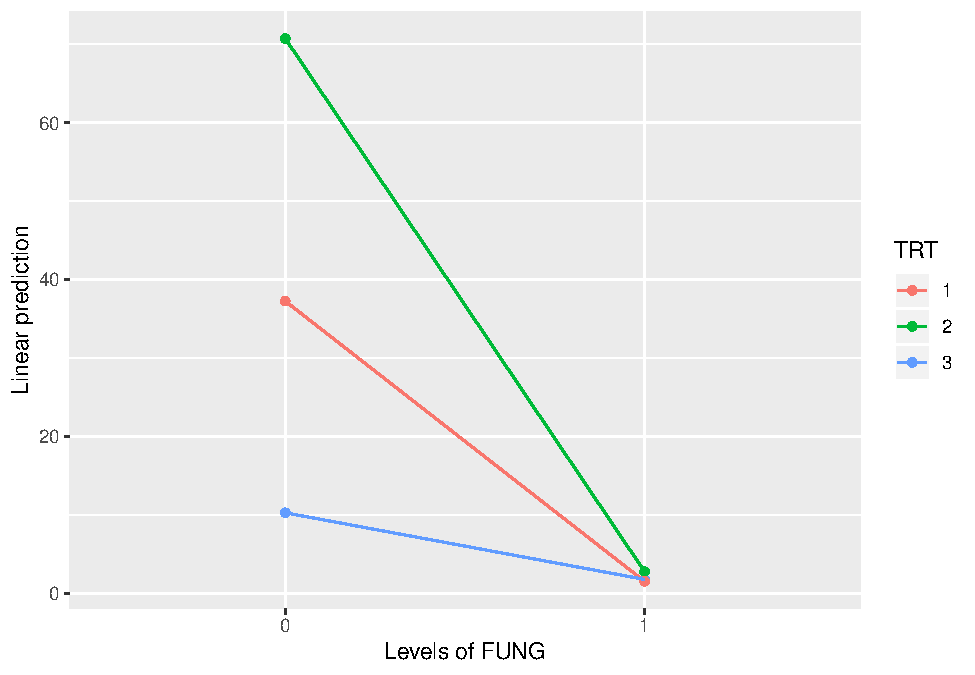
\includegraphics{04-ex_yield_loss_files/figure-latex/mixed-model-DS-1.pdf}

\begin{Shaded}
\begin{Highlighting}[]
\CommentTok{# to do anova for random effects, we need to compare mm_1 with a model that only has fixed effects,}
\CommentTok{# we can use `gls()` function in `nlme` to fit the fixed effects model}
\NormalTok{fixed_model <-}\StringTok{ }\KeywordTok{gls}\NormalTok{(DS }\OperatorTok{~}\StringTok{ }\NormalTok{TRT }\OperatorTok{*}\StringTok{ }\NormalTok{FUNG,}
                                     \DataTypeTok{data =}\NormalTok{ a)}

\CommentTok{# test the random effects in the model}
\KeywordTok{anova}\NormalTok{(mm_}\DecValTok{1}\NormalTok{, fixed_model)}
\end{Highlighting}
\end{Shaded}

\begin{verbatim}
##             Model df      AIC      BIC    logLik   Test      L.Ratio
## mm_1            1  9 156.1691 164.1825 -69.08456                    
## fixed_model     2  7 152.1691 158.4017 -69.08456 1 vs 2 1.250038e-08
##             p-value
## mm_1               
## fixed_model       1
\end{verbatim}

\begin{Shaded}
\begin{Highlighting}[]
\CommentTok{# least square means}
\KeywordTok{test}\NormalTok{(}\KeywordTok{emmeans}\NormalTok{(mm_}\DecValTok{1}\NormalTok{, }\StringTok{"TRT"}\NormalTok{))}
\end{Highlighting}
\end{Shaded}

\begin{verbatim}
## NOTE: Results may be misleading due to involvement in interactions
\end{verbatim}

\begin{verbatim}
##  TRT emmean  SE df t.ratio p.value
##  1     19.4 2.8  3  6.920  0.0062 
##  2     36.8 2.8  3 13.126  0.0010 
##  3      6.0 2.8  3  2.143  0.1215 
## 
## Results are averaged over the levels of: FUNG 
## d.f. method: containment
\end{verbatim}

\begin{Shaded}
\begin{Highlighting}[]
\KeywordTok{test}\NormalTok{(}\KeywordTok{emmeans}\NormalTok{(mm_}\DecValTok{1}\NormalTok{, }\StringTok{"FUNG"}\NormalTok{))}
\end{Highlighting}
\end{Shaded}

\begin{verbatim}
## NOTE: Results may be misleading due to involvement in interactions
\end{verbatim}

\begin{verbatim}
##  FUNG emmean   SE df t.ratio p.value
##  0      39.4 2.29  3 17.243  0.0004 
##  1       2.0 2.29  3  0.875  0.4460 
## 
## Results are averaged over the levels of: TRT 
## d.f. method: containment
\end{verbatim}

\begin{Shaded}
\begin{Highlighting}[]
\CommentTok{# pairwise difference}
\KeywordTok{test}\NormalTok{(}\KeywordTok{emmeans}\NormalTok{(mm_}\DecValTok{1}\NormalTok{, pairwise }\OperatorTok{~}\StringTok{ }\NormalTok{TRT), }\DataTypeTok{adjust =} \StringTok{"none"}\NormalTok{)}
\end{Highlighting}
\end{Shaded}

\begin{verbatim}
## NOTE: Results may be misleading due to involvement in interactions
\end{verbatim}

\begin{verbatim}
## $emmeans
##  TRT emmean  SE df t.ratio p.value
##  1     19.4 2.8  3  6.920  0.0062 
##  2     36.8 2.8  3 13.126  0.0010 
##  3      6.0 2.8  3  2.143  0.1215 
## 
## Results are averaged over the levels of: FUNG 
## d.f. method: containment 
## 
## $contrasts
##  contrast estimate   SE df t.ratio p.value
##  1 - 2       -17.4 3.96  6 -4.388  0.0046 
##  1 - 3        13.4 3.96  6  3.378  0.0149 
##  2 - 3        30.8 3.96  6  7.766  0.0002 
## 
## Results are averaged over the levels of: FUNG
\end{verbatim}

\begin{Shaded}
\begin{Highlighting}[]
\KeywordTok{test}\NormalTok{(}\KeywordTok{emmeans}\NormalTok{(mm_}\DecValTok{1}\NormalTok{, pairwise }\OperatorTok{~}\StringTok{ }\NormalTok{FUNG))}
\end{Highlighting}
\end{Shaded}

\begin{verbatim}
## NOTE: Results may be misleading due to involvement in interactions
\end{verbatim}

\begin{verbatim}
## $emmeans
##  FUNG emmean   SE df t.ratio p.value
##  0      39.4 2.29  3 17.243  0.0004 
##  1       2.0 2.29  3  0.875  0.4460 
## 
## Results are averaged over the levels of: TRT 
## d.f. method: containment 
## 
## $contrasts
##  contrast estimate   SE df t.ratio p.value
##  0 - 1        37.4 3.23  9 11.574  <.0001 
## 
## Results are averaged over the levels of: TRT
\end{verbatim}

\begin{Shaded}
\begin{Highlighting}[]
\KeywordTok{test}\NormalTok{(}\KeywordTok{emmeans}\NormalTok{(mm_}\DecValTok{1}\NormalTok{, pairwise }\OperatorTok{~}\StringTok{ }\NormalTok{TRT}\OperatorTok{*}\NormalTok{FUNG), }\DataTypeTok{adjust =} \StringTok{"none"}\NormalTok{)}
\end{Highlighting}
\end{Shaded}

\begin{verbatim}
## $emmeans
##  TRT FUNG emmean   SE df t.ratio p.value
##  1   0     37.25 3.96  3  9.408  0.0025 
##  2   0     70.75 3.96  3 17.869  0.0004 
##  3   0     10.25 3.96  3  2.589  0.0812 
##  1   1      1.50 3.96  3  0.379  0.7300 
##  2   1      2.75 3.96  3  0.695  0.5373 
##  3   1      1.75 3.96  3  0.442  0.6884 
## 
## d.f. method: containment 
## 
## $contrasts
##  contrast  estimate  SE df t.ratio p.value
##  1,0 - 2,0   -33.50 5.6  6 -5.983  0.0010 
##  1,0 - 3,0    27.00 5.6  6  4.822  0.0029 
##  1,0 - 1,1    35.75 5.6  9  6.385  0.0001 
##  1,0 - 2,1    34.50 5.6  6  6.161  0.0008 
##  1,0 - 3,1    35.50 5.6  6  6.340  0.0007 
##  2,0 - 3,0    60.50 5.6  6 10.805  <.0001 
##  2,0 - 1,1    69.25 5.6  6 12.367  <.0001 
##  2,0 - 2,1    68.00 5.6  9 12.144  <.0001 
##  2,0 - 3,1    69.00 5.6  6 12.323  <.0001 
##  3,0 - 1,1     8.75 5.6  6  1.563  0.1692 
##  3,0 - 2,1     7.50 5.6  6  1.339  0.2289 
##  3,0 - 3,1     8.50 5.6  9  1.518  0.1633 
##  1,1 - 2,1    -1.25 5.6  6 -0.223  0.8308 
##  1,1 - 3,1    -0.25 5.6  6 -0.045  0.9658 
##  2,1 - 3,1     1.00 5.6  6  0.179  0.8641
\end{verbatim}

\hypertarget{diagnostic-plots-1}{%
\subsection{Diagnostic plots}\label{diagnostic-plots-1}}

\begin{Shaded}
\begin{Highlighting}[]
\CommentTok{# pearson residuals vs. fitted values}
\KeywordTok{plot}\NormalTok{(mm_}\DecValTok{1}\NormalTok{, }\KeywordTok{resid}\NormalTok{(., }\DataTypeTok{type=}\StringTok{"pearson"}\NormalTok{) }\OperatorTok{~}\StringTok{ }\KeywordTok{fitted}\NormalTok{(.), }\DataTypeTok{abline =} \DecValTok{0}\NormalTok{)}
\end{Highlighting}
\end{Shaded}

\includegraphics{04-ex_yield_loss_files/figure-latex/diagnostic-plots-1.pdf}

\begin{Shaded}
\begin{Highlighting}[]
\CommentTok{# standardaized residuals vs. fitted values}
\KeywordTok{plot}\NormalTok{(mm_}\DecValTok{1}\NormalTok{, }\KeywordTok{resid}\NormalTok{(., }\DataTypeTok{scaled=}\OtherTok{TRUE}\NormalTok{) }\OperatorTok{~}\StringTok{ }\KeywordTok{fitted}\NormalTok{(.), }\DataTypeTok{abline =} \DecValTok{0}\NormalTok{)}
\end{Highlighting}
\end{Shaded}

\includegraphics{04-ex_yield_loss_files/figure-latex/diagnostic-plots-2.pdf}

\begin{Shaded}
\begin{Highlighting}[]
\CommentTok{# qq plot}
\KeywordTok{qqnorm}\NormalTok{(}\KeywordTok{residuals}\NormalTok{(mm_}\DecValTok{1}\NormalTok{))}
\KeywordTok{qqline}\NormalTok{(}\KeywordTok{residuals}\NormalTok{(mm_}\DecValTok{1}\NormalTok{))}
\end{Highlighting}
\end{Shaded}

\includegraphics{04-ex_yield_loss_files/figure-latex/diagnostic-plots-3.pdf}

\begin{Shaded}
\begin{Highlighting}[]
\CommentTok{#observed vs. fitted values}
\KeywordTok{plot}\NormalTok{(mm_}\DecValTok{1}\NormalTok{, DS }\OperatorTok{~}\StringTok{ }\KeywordTok{fitted}\NormalTok{(.), }\DataTypeTok{abline =} \KeywordTok{c}\NormalTok{(}\DecValTok{0}\NormalTok{,}\DecValTok{1}\NormalTok{))}
\end{Highlighting}
\end{Shaded}

\includegraphics{04-ex_yield_loss_files/figure-latex/diagnostic-plots-4.pdf}

\hypertarget{mixed-model-for-response-variable-yield}{%
\section{Mixed model for response variable YIELD}\label{mixed-model-for-response-variable-yield}}

\begin{Shaded}
\begin{Highlighting}[]
\CommentTok{# fit the model  }
\NormalTok{mm_}\DecValTok{2}\NormalTok{ <-}\StringTok{ }\KeywordTok{lme}\NormalTok{(YIELD }\OperatorTok{~}\StringTok{ }\NormalTok{TRT}\OperatorTok{*}\NormalTok{FUNG, }\CommentTok{# fixed effects}
            \DataTypeTok{data =}\NormalTok{ a,}
            \DataTypeTok{random =} \OperatorTok{~}\DecValTok{1}\OperatorTok{|}\NormalTok{BLK}\OperatorTok{/}\NormalTok{TRT) }\CommentTok{# read mm_2 as mixed model 2}

\CommentTok{# summary output}
\KeywordTok{summary}\NormalTok{(mm_}\DecValTok{2}\NormalTok{)}
\end{Highlighting}
\end{Shaded}

\begin{verbatim}
## Linear mixed-effects model fit by REML
##  Data: a 
##        AIC      BIC   logLik
##   209.9214 217.9348 -95.9607
## 
## Random effects:
##  Formula: ~1 | BLK
##         (Intercept)
## StdDev:    11.99815
## 
##  Formula: ~1 | TRT %in% BLK
##         (Intercept) Residual
## StdDev: 0.001914579 33.61779
## 
## Fixed effects: YIELD ~ TRT * FUNG 
##                 Value Std.Error DF  t-value p-value
## (Intercept)  335.1667  9.114752  9 36.77189  0.0000
## TRT.L         21.3016 11.885682  6  1.79221  0.1233
## TRT.Q         54.5522 11.885682  6  4.58974  0.0037
## FUNG.L        93.9274  9.704619  9  9.67862  0.0000
## TRT.L:FUNG.L -31.8750 16.808893  9 -1.89632  0.0904
## TRT.Q:FUNG.L -75.2720 16.808893  9 -4.47811  0.0015
##  Correlation: 
##              (Intr) TRT.L TRT.Q FUNG.L TRT.L:
## TRT.L        0                               
## TRT.Q        0      0                        
## FUNG.L       0      0     0                  
## TRT.L:FUNG.L 0      0     0     0            
## TRT.Q:FUNG.L 0      0     0     0      0     
## 
## Standardized Within-Group Residuals:
##         Min          Q1         Med          Q3         Max 
## -2.04399017 -0.33265713  0.07191314  0.49972251  1.20545632 
## 
## Number of Observations: 24
## Number of Groups: 
##          BLK TRT %in% BLK 
##            4           12
\end{verbatim}

\begin{Shaded}
\begin{Highlighting}[]
\CommentTok{# type 3 tests of fixed effects}
\KeywordTok{anova}\NormalTok{(mm_}\DecValTok{2}\NormalTok{)}
\end{Highlighting}
\end{Shaded}

\begin{verbatim}
##             numDF denDF   F-value p-value
## (Intercept)     1     9 1352.1720  <.0001
## TRT             2     6   12.1389  0.0078
## FUNG            1     9   93.6757  <.0001
## TRT:FUNG        2     9   11.8247  0.0030
\end{verbatim}

\begin{Shaded}
\begin{Highlighting}[]
\CommentTok{# visualize interaction}
\KeywordTok{emmip}\NormalTok{(mm_}\DecValTok{2}\NormalTok{, TRT }\OperatorTok{~}\StringTok{ }\NormalTok{FUNG)}
\end{Highlighting}
\end{Shaded}

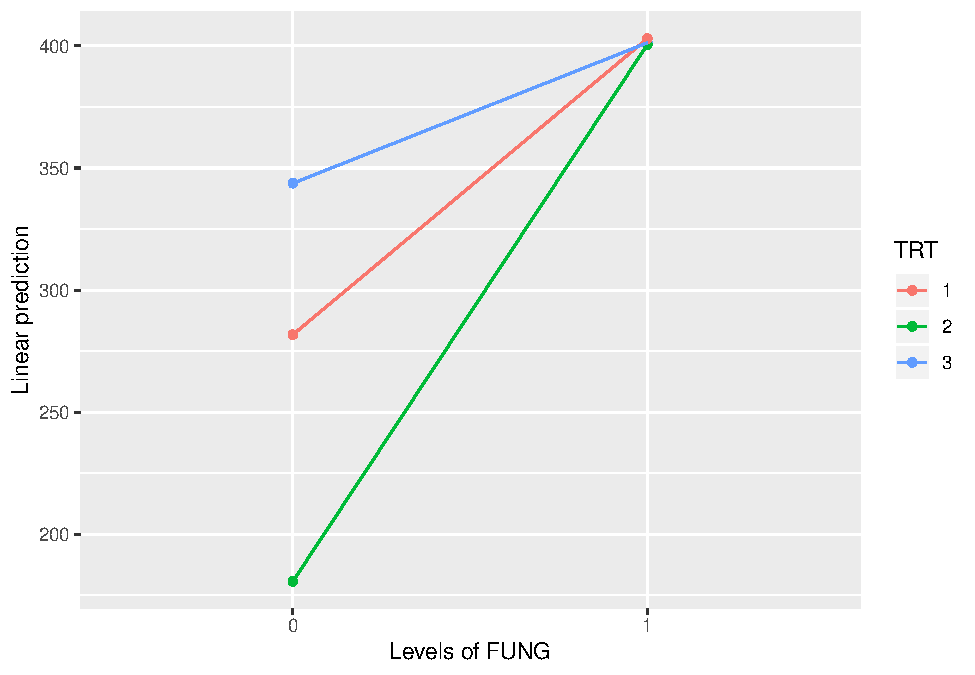
\includegraphics{04-ex_yield_loss_files/figure-latex/mixed-model-yield-1.pdf}

\begin{Shaded}
\begin{Highlighting}[]
\CommentTok{# to do anova for random effects, we need to compare mm_1 with a model that only has fixed effects,}
\CommentTok{# we can use `gls()` function in `nlme` to fit the fixed effects model}
\NormalTok{fixed_model_YIELD <-}\StringTok{ }\KeywordTok{gls}\NormalTok{(YIELD }\OperatorTok{~}\StringTok{ }\NormalTok{TRT }\OperatorTok{*}\StringTok{ }\NormalTok{FUNG,}
                                     \DataTypeTok{data =}\NormalTok{ a)}

\CommentTok{# test the random effects in the model}
\KeywordTok{anova}\NormalTok{(mm_}\DecValTok{2}\NormalTok{, fixed_model_YIELD)}
\end{Highlighting}
\end{Shaded}

\begin{verbatim}
##                   Model df      AIC      BIC    logLik   Test   L.Ratio
## mm_2                  1  9 209.9214 217.9348 -95.96070                 
## fixed_model_YIELD     2  7 206.3763 212.6089 -96.18815 1 vs 2 0.4548877
##                   p-value
## mm_2                     
## fixed_model_YIELD  0.7966
\end{verbatim}

\begin{Shaded}
\begin{Highlighting}[]
\CommentTok{# least square means}
\KeywordTok{test}\NormalTok{(}\KeywordTok{emmeans}\NormalTok{(mm_}\DecValTok{2}\NormalTok{, }\StringTok{"TRT"}\NormalTok{))}
\end{Highlighting}
\end{Shaded}

\begin{verbatim}
## NOTE: Results may be misleading due to involvement in interactions
\end{verbatim}

\begin{verbatim}
##  TRT emmean   SE df t.ratio p.value
##  1      342 13.3  3 25.716  0.0001 
##  2      291 13.3  3 21.829  0.0002 
##  3      372 13.3  3 27.978  0.0001 
## 
## Results are averaged over the levels of: FUNG 
## d.f. method: containment
\end{verbatim}

\begin{Shaded}
\begin{Highlighting}[]
\KeywordTok{test}\NormalTok{(}\KeywordTok{emmeans}\NormalTok{(mm_}\DecValTok{2}\NormalTok{, }\StringTok{"FUNG"}\NormalTok{))}
\end{Highlighting}
\end{Shaded}

\begin{verbatim}
## NOTE: Results may be misleading due to involvement in interactions
\end{verbatim}

\begin{verbatim}
##  FUNG emmean   SE df t.ratio p.value
##  0       269 11.4  3 23.556  0.0002 
##  1       402 11.4  3 35.198  0.0001 
## 
## Results are averaged over the levels of: TRT 
## d.f. method: containment
\end{verbatim}

\begin{Shaded}
\begin{Highlighting}[]
\CommentTok{# pairwise difference}
\KeywordTok{test}\NormalTok{(}\KeywordTok{emmeans}\NormalTok{(mm_}\DecValTok{2}\NormalTok{, pairwise }\OperatorTok{~}\StringTok{ }\NormalTok{TRT), }\DataTypeTok{adjust =} \StringTok{"none"}\NormalTok{)}
\end{Highlighting}
\end{Shaded}

\begin{verbatim}
## NOTE: Results may be misleading due to involvement in interactions
\end{verbatim}

\begin{verbatim}
## $emmeans
##  TRT emmean   SE df t.ratio p.value
##  1      342 13.3  3 25.716  0.0001 
##  2      291 13.3  3 21.829  0.0002 
##  3      372 13.3  3 27.978  0.0001 
## 
## Results are averaged over the levels of: FUNG 
## d.f. method: containment 
## 
## $contrasts
##  contrast estimate   SE df t.ratio p.value
##  1 - 2        51.8 16.8  6  3.079  0.0217 
##  1 - 3       -30.1 16.8  6 -1.792  0.1233 
##  2 - 3       -81.9 16.8  6 -4.871  0.0028 
## 
## Results are averaged over the levels of: FUNG
\end{verbatim}

\begin{Shaded}
\begin{Highlighting}[]
\KeywordTok{test}\NormalTok{(}\KeywordTok{emmeans}\NormalTok{(mm_}\DecValTok{2}\NormalTok{, pairwise }\OperatorTok{~}\StringTok{ }\NormalTok{FUNG))}
\end{Highlighting}
\end{Shaded}

\begin{verbatim}
## NOTE: Results may be misleading due to involvement in interactions
\end{verbatim}

\begin{verbatim}
## $emmeans
##  FUNG emmean   SE df t.ratio p.value
##  0       269 11.4  3 23.556  0.0002 
##  1       402 11.4  3 35.198  0.0001 
## 
## Results are averaged over the levels of: TRT 
## d.f. method: containment 
## 
## $contrasts
##  contrast estimate   SE df t.ratio p.value
##  0 - 1        -133 13.7  9 -9.679  <.0001 
## 
## Results are averaged over the levels of: TRT
\end{verbatim}

\begin{Shaded}
\begin{Highlighting}[]
\KeywordTok{test}\NormalTok{(}\KeywordTok{emmeans}\NormalTok{(mm_}\DecValTok{2}\NormalTok{, pairwise }\OperatorTok{~}\StringTok{ }\NormalTok{TRT}\OperatorTok{*}\NormalTok{FUNG), }\DataTypeTok{adjust =} \StringTok{"none"}\NormalTok{)}
\end{Highlighting}
\end{Shaded}

\begin{verbatim}
## $emmeans
##  TRT FUNG emmean   SE df t.ratio p.value
##  1   0       282 17.8  3 15.787  0.0006 
##  2   0       181 17.8  3 10.128  0.0021 
##  3   0       344 17.8  3 19.261  0.0003 
##  1   1       403 17.8  3 22.580  0.0002 
##  2   1       400 17.8  3 22.440  0.0002 
##  3   1       401 17.8  3 22.482  0.0002 
## 
## d.f. method: containment 
## 
## $contrasts
##  contrast  estimate   SE df t.ratio p.value
##  1,0 - 2,0   101.00 23.8  6  4.249  0.0054 
##  1,0 - 3,0   -62.00 23.8  6 -2.608  0.0402 
##  1,0 - 1,1  -121.25 23.8  9 -5.101  0.0006 
##  1,0 - 2,1  -118.75 23.8  6 -4.996  0.0025 
##  1,0 - 3,1  -119.50 23.8  6 -5.027  0.0024 
##  2,0 - 3,0  -163.00 23.8  6 -6.857  0.0005 
##  2,0 - 1,1  -222.25 23.8  6 -9.349  0.0001 
##  2,0 - 2,1  -219.75 23.8  9 -9.244  <.0001 
##  2,0 - 3,1  -220.50 23.8  6 -9.276  0.0001 
##  3,0 - 1,1   -59.25 23.8  6 -2.492  0.0470 
##  3,0 - 2,1   -56.75 23.8  6 -2.387  0.0542 
##  3,0 - 3,1   -57.50 23.8  9 -2.419  0.0387 
##  1,1 - 2,1     2.50 23.8  6  0.105  0.9197 
##  1,1 - 3,1     1.75 23.8  6  0.074  0.9437 
##  2,1 - 3,1    -0.75 23.8  6 -0.032  0.9759
\end{verbatim}

\hypertarget{diagnostic-plots-2}{%
\subsection{Diagnostic plots}\label{diagnostic-plots-2}}

\begin{Shaded}
\begin{Highlighting}[]
\CommentTok{# pearson residuals vs. fitted values}
\KeywordTok{plot}\NormalTok{(mm_}\DecValTok{2}\NormalTok{, }\KeywordTok{resid}\NormalTok{(., }\DataTypeTok{type=}\StringTok{"pearson"}\NormalTok{) }\OperatorTok{~}\StringTok{ }\KeywordTok{fitted}\NormalTok{(.), }\DataTypeTok{abline =} \DecValTok{0}\NormalTok{)}
\end{Highlighting}
\end{Shaded}

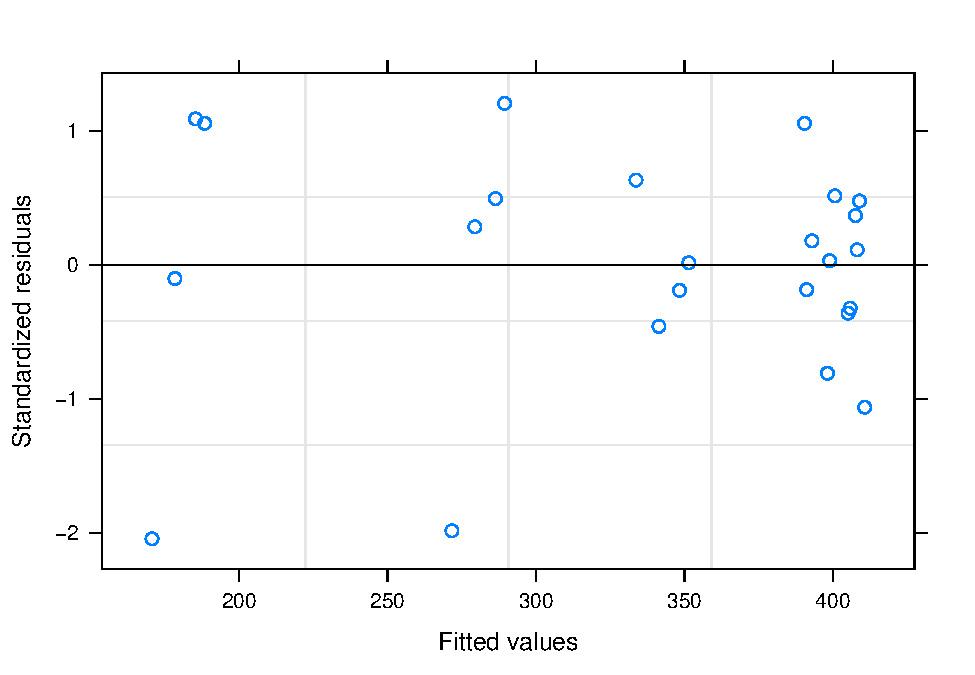
\includegraphics{04-ex_yield_loss_files/figure-latex/diagnostic-plots-yield-1.pdf}

\begin{Shaded}
\begin{Highlighting}[]
\CommentTok{# standardaized residuals vs. fitted values}
\KeywordTok{plot}\NormalTok{(mm_}\DecValTok{2}\NormalTok{, }\KeywordTok{resid}\NormalTok{(., }\DataTypeTok{scaled=}\OtherTok{TRUE}\NormalTok{) }\OperatorTok{~}\StringTok{ }\KeywordTok{fitted}\NormalTok{(.), }\DataTypeTok{abline =} \DecValTok{0}\NormalTok{)}
\end{Highlighting}
\end{Shaded}

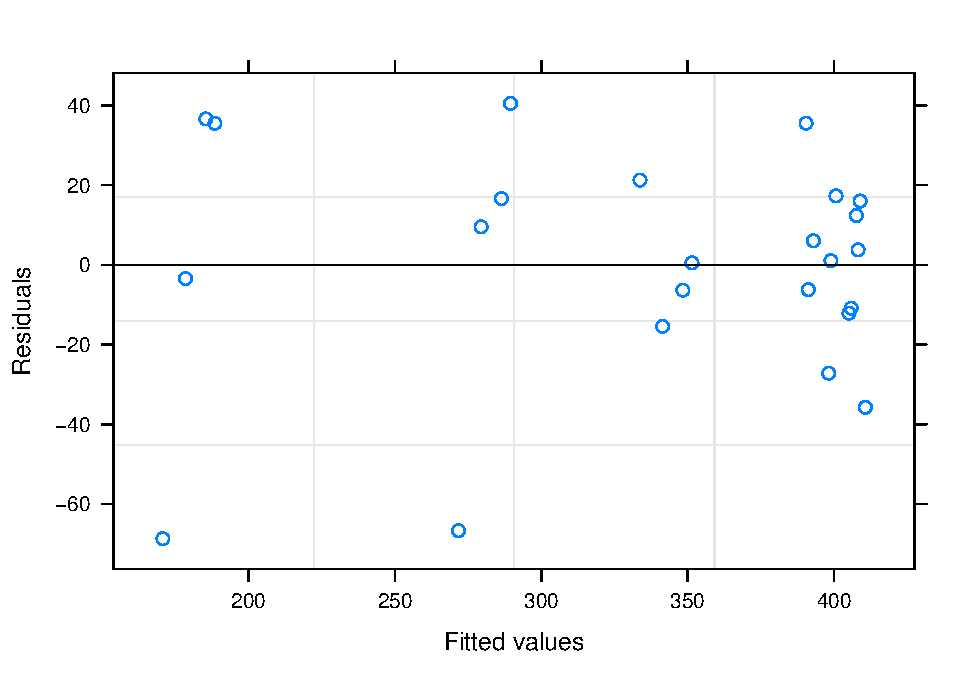
\includegraphics{04-ex_yield_loss_files/figure-latex/diagnostic-plots-yield-2.pdf}

\begin{Shaded}
\begin{Highlighting}[]
\CommentTok{# qq plot}
\KeywordTok{qqnorm}\NormalTok{(}\KeywordTok{residuals}\NormalTok{(mm_}\DecValTok{2}\NormalTok{))}
\KeywordTok{qqline}\NormalTok{(}\KeywordTok{residuals}\NormalTok{(mm_}\DecValTok{2}\NormalTok{))}
\end{Highlighting}
\end{Shaded}

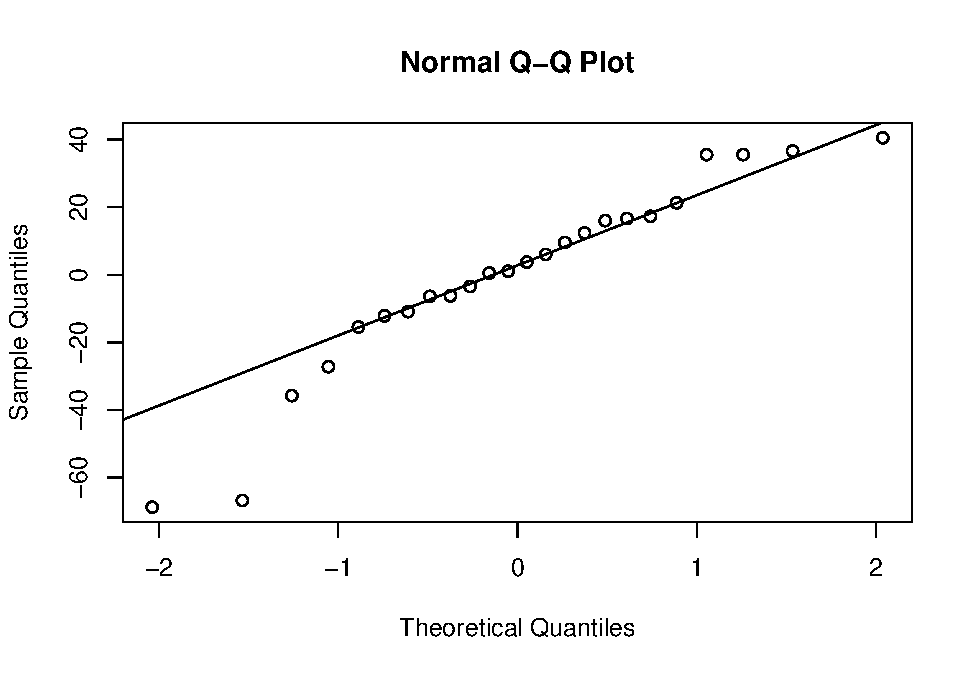
\includegraphics{04-ex_yield_loss_files/figure-latex/diagnostic-plots-yield-3.pdf}

\begin{Shaded}
\begin{Highlighting}[]
\CommentTok{#observed vs. fitted values}
\KeywordTok{plot}\NormalTok{(mm_}\DecValTok{2}\NormalTok{, YIELD }\OperatorTok{~}\StringTok{ }\KeywordTok{fitted}\NormalTok{(.), }\DataTypeTok{abline =} \KeywordTok{c}\NormalTok{(}\DecValTok{0}\NormalTok{,}\DecValTok{1}\NormalTok{))}
\end{Highlighting}
\end{Shaded}

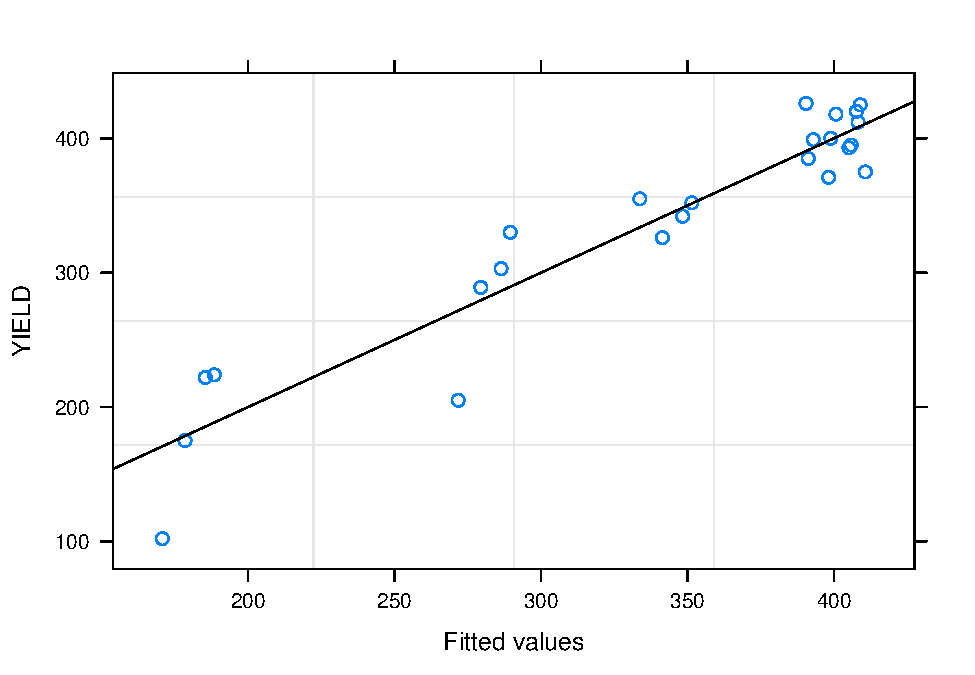
\includegraphics{04-ex_yield_loss_files/figure-latex/diagnostic-plots-yield-4.pdf}

\hypertarget{linear-regression-between-yield-and-ds}{%
\section{Linear regression between YIELD and DS}\label{linear-regression-between-yield-and-ds}}

\begin{Shaded}
\begin{Highlighting}[]
\CommentTok{# fit `lm` model}
\NormalTok{lm_}\DecValTok{1}\NormalTok{ <-}\StringTok{ }\KeywordTok{lm}\NormalTok{(YIELD }\OperatorTok{~}\StringTok{ }\NormalTok{DS, }\DataTypeTok{data =}\NormalTok{ a) }
\KeywordTok{summary}\NormalTok{(lm_}\DecValTok{1}\NormalTok{)}
\end{Highlighting}
\end{Shaded}

\begin{verbatim}
## 
## Call:
## lm(formula = YIELD ~ DS, data = a)
## 
## Residuals:
##     Min      1Q  Median      3Q     Max 
## -61.196 -18.565   0.856  22.676  56.812 
## 
## Coefficients:
##             Estimate Std. Error t value Pr(>|t|)    
## (Intercept) 399.2384     8.0711   49.47  < 2e-16 ***
## DS           -3.0940     0.2399  -12.90 9.81e-12 ***
## ---
## Signif. codes:  0 '***' 0.001 '**' 0.01 '*' 0.05 '.' 0.1 ' ' 1
## 
## Residual standard error: 31.17 on 22 degrees of freedom
## Multiple R-squared:  0.8832, Adjusted R-squared:  0.8779 
## F-statistic: 166.4 on 1 and 22 DF,  p-value: 9.809e-12
\end{verbatim}

\begin{Shaded}
\begin{Highlighting}[]
\KeywordTok{anova}\NormalTok{(lm_}\DecValTok{1}\NormalTok{)}
\end{Highlighting}
\end{Shaded}

\begin{verbatim}
## Analysis of Variance Table
## 
## Response: YIELD
##           Df Sum Sq Mean Sq F value    Pr(>F)    
## DS         1 161600  161600  166.38 9.809e-12 ***
## Residuals 22  21368     971                      
## ---
## Signif. codes:  0 '***' 0.001 '**' 0.01 '*' 0.05 '.' 0.1 ' ' 1
\end{verbatim}

\begin{Shaded}
\begin{Highlighting}[]
\CommentTok{# diagnostic plots  }
\KeywordTok{residplot}\NormalTok{(lm_}\DecValTok{1}\NormalTok{)}
\end{Highlighting}
\end{Shaded}

\hypertarget{linear-regression-between-ry1-and-ds}{%
\subsection{Linear regression between RY1 and DS}\label{linear-regression-between-ry1-and-ds}}

\begin{Shaded}
\begin{Highlighting}[]
\NormalTok{b <-}\StringTok{ }\NormalTok{a }\OperatorTok\StringTok{ }
\StringTok{    }\KeywordTok{mutate}\NormalTok{(}\DataTypeTok{RY1 =}\NormalTok{ YIELD}\OperatorTok{/}\FloatTok{399.23843}\NormalTok{)}

\CommentTok{# fit linear regression model}
\NormalTok{lm_}\DecValTok{2}\NormalTok{ <-}\StringTok{ }\KeywordTok{lm}\NormalTok{(RY1 }\OperatorTok{~}\StringTok{ }\NormalTok{DS, }\DataTypeTok{data =}\NormalTok{ b)}
\KeywordTok{summary}\NormalTok{(lm_}\DecValTok{2}\NormalTok{)}
\end{Highlighting}
\end{Shaded}

\begin{verbatim}
## 
## Call:
## lm(formula = RY1 ~ DS, data = b)
## 
## Residuals:
##       Min        1Q    Median        3Q       Max 
## -0.153282 -0.046502  0.002143  0.056798  0.142301 
## 
## Coefficients:
##               Estimate Std. Error t value Pr(>|t|)    
## (Intercept)  1.0000000  0.0202162   49.47  < 2e-16 ***
## DS          -0.0077498  0.0006008  -12.90 9.81e-12 ***
## ---
## Signif. codes:  0 '***' 0.001 '**' 0.01 '*' 0.05 '.' 0.1 ' ' 1
## 
## Residual standard error: 0.07806 on 22 degrees of freedom
## Multiple R-squared:  0.8832, Adjusted R-squared:  0.8779 
## F-statistic: 166.4 on 1 and 22 DF,  p-value: 9.809e-12
\end{verbatim}

\begin{Shaded}
\begin{Highlighting}[]
\KeywordTok{anova}\NormalTok{(lm_}\DecValTok{2}\NormalTok{)}
\end{Highlighting}
\end{Shaded}

\begin{verbatim}
## Analysis of Variance Table
## 
## Response: RY1
##           Df  Sum Sq Mean Sq F value    Pr(>F)    
## DS         1 1.01385 1.01385  166.38 9.809e-12 ***
## Residuals 22 0.13406 0.00609                      
## ---
## Signif. codes:  0 '***' 0.001 '**' 0.01 '*' 0.05 '.' 0.1 ' ' 1
\end{verbatim}

\begin{Shaded}
\begin{Highlighting}[]
\CommentTok{# diagnostic plots  }
\KeywordTok{residplot}\NormalTok{(lm_}\DecValTok{2}\NormalTok{)}
\end{Highlighting}
\end{Shaded}

\hypertarget{transform-dataset-a}{%
\subsection{Transform dataset a}\label{transform-dataset-a}}

\begin{Shaded}
\begin{Highlighting}[]
\NormalTok{a_yield <-}\StringTok{ }\NormalTok{a }\OperatorTok\StringTok{ }
\StringTok{    }\NormalTok{dplyr}\OperatorTok{::}\KeywordTok{select}\NormalTok{(BLK, TRT, YIELD) }\OperatorTok\StringTok{ }
\StringTok{    }\KeywordTok{arrange}\NormalTok{(BLK, TRT, YIELD) }\OperatorTok\StringTok{ }
\StringTok{    }\KeywordTok{group_by}\NormalTok{(BLK, TRT) }\OperatorTok\StringTok{ }
\StringTok{    }\KeywordTok{summarise}\NormalTok{(}\DataTypeTok{RY2 =}\NormalTok{ YIELD[}\DecValTok{1}\NormalTok{]}\OperatorTok{/}\NormalTok{YIELD[}\DecValTok{2}\NormalTok{]) }\OperatorTok\StringTok{ }
\StringTok{    }\KeywordTok{ungroup}\NormalTok{()}


\NormalTok{a_ds <-}\StringTok{ }\NormalTok{a }\OperatorTok\StringTok{ }
\StringTok{    }\NormalTok{dplyr}\OperatorTok{::}\KeywordTok{select}\NormalTok{(BLK, TRT, DS) }\OperatorTok\StringTok{ }
\StringTok{    }\KeywordTok{arrange}\NormalTok{(BLK, TRT, DS) }\OperatorTok\StringTok{ }
\StringTok{    }\KeywordTok{group_by}\NormalTok{(BLK, TRT) }\OperatorTok\StringTok{ }
\StringTok{    }\KeywordTok{summarise}\NormalTok{(}\DataTypeTok{CDS =}\NormalTok{ DS[}\DecValTok{2}\NormalTok{]) }\OperatorTok\StringTok{ }
\StringTok{    }\KeywordTok{ungroup}\NormalTok{()}

\NormalTok{a_new <-}\StringTok{ }\NormalTok{a_yield }\OperatorTok\StringTok{ }
\StringTok{    }\KeywordTok{inner_join}\NormalTok{(a_ds) }\OperatorTok\StringTok{ }
\StringTok{    }\KeywordTok{ungroup}\NormalTok{() }\OperatorTok\StringTok{ }
\StringTok{    }\KeywordTok{mutate}\NormalTok{(}\DataTypeTok{BLK =} \KeywordTok{parse_factor}\NormalTok{(}\KeywordTok{as.character}\NormalTok{(BLK)),}
                 \DataTypeTok{TRT =} \KeywordTok{parse_factor}\NormalTok{(}\KeywordTok{as.character}\NormalTok{(TRT)))}
\end{Highlighting}
\end{Shaded}

\begin{verbatim}
## Joining, by = c("BLK", "TRT")
\end{verbatim}

\begin{Shaded}
\begin{Highlighting}[]
\CommentTok{# print the data}
\NormalTok{a_new}
\end{Highlighting}
\end{Shaded}

\begin{verbatim}
## # A tibble: 12 x 4
##    BLK   TRT     RY2   CDS
##    <fct> <fct> <dbl> <dbl>
##  1 1     1     0.514    43
##  2 1     2     0.239    92
##  3 1     3     0.922     7
##  4 2     1     0.88     27
##  5 2     2     0.544    75
##  6 2     3     0.828    10
##  7 3     1     0.721    47
##  8 3     2     0.565    63
##  9 3     3     0.866    12
## 10 4     1     0.691    32
## 11 4     2     0.472    53
## 12 4     3     0.815    12
\end{verbatim}

\hypertarget{mixed-model-for-ry2}{%
\section{Mixed model for RY2}\label{mixed-model-for-ry2}}

\begin{Shaded}
\begin{Highlighting}[]
\CommentTok{# fit the model  }
\NormalTok{mm_}\DecValTok{3}\NormalTok{ <-}\StringTok{ }\KeywordTok{lme}\NormalTok{(RY2 }\OperatorTok{~}\StringTok{ }\NormalTok{TRT, }\CommentTok{# fixed effects}
            \DataTypeTok{data =}\NormalTok{ a_new,}
            \DataTypeTok{random =} \OperatorTok{~}\DecValTok{1}\OperatorTok{|}\NormalTok{BLK) }\CommentTok{# read mm_3 as mixed model 3}

\CommentTok{# summary output}
\KeywordTok{summary}\NormalTok{(mm_}\DecValTok{3}\NormalTok{)}
\end{Highlighting}
\end{Shaded}

\begin{verbatim}
## Linear mixed-effects model fit by REML
##  Data: a_new 
##       AIC      BIC   logLik
##   2.04077 3.026893 3.979615
## 
## Random effects:
##  Formula: ~1 | BLK
##         (Intercept)  Residual
## StdDev:  0.05297273 0.1134963
## 
## Fixed effects: RY2 ~ TRT 
##                  Value  Std.Error DF   t-value p-value
## (Intercept)  0.7016501 0.06262490  6 11.204012  0.0000
## TRT2        -0.2467228 0.08025398  6 -3.074274  0.0218
## TRT3         0.1561339 0.08025398  6  1.945497  0.0997
##  Correlation: 
##      (Intr) TRT2  
## TRT2 -0.641       
## TRT3 -0.641  0.500
## 
## Standardized Within-Group Residuals:
##         Min          Q1         Med          Q3         Max 
## -1.50508335 -0.38516867 -0.01698779  0.58195830  1.29565814 
## 
## Number of Observations: 12
## Number of Groups: 4
\end{verbatim}

\begin{Shaded}
\begin{Highlighting}[]
\CommentTok{# type 3 tests of fixed effects}
\KeywordTok{anova}\NormalTok{(mm_}\DecValTok{3}\NormalTok{)}
\end{Highlighting}
\end{Shaded}

\begin{verbatim}
##             numDF denDF   F-value p-value
## (Intercept)     1     6 254.00333  <.0001
## TRT             2     6  12.81141  0.0068
\end{verbatim}

\begin{Shaded}
\begin{Highlighting}[]
\CommentTok{# to do anova for random effects, we need to compare mm_1 with a model that only has fixed effects,}
\CommentTok{# we can use `gls()` function in `nlme` to fit the fixed effects model}
\NormalTok{fixed_model_RY2 <-}\StringTok{ }\KeywordTok{gls}\NormalTok{(RY2 }\OperatorTok{~}\StringTok{ }\NormalTok{TRT,}
                                     \DataTypeTok{data =}\NormalTok{ a_new)}

\CommentTok{# test the random effects in the model}
\KeywordTok{anova}\NormalTok{(mm_}\DecValTok{3}\NormalTok{, fixed_model_RY2)}
\end{Highlighting}
\end{Shaded}

\begin{verbatim}
##                 Model df       AIC      BIC   logLik   Test   L.Ratio
## mm_3                1  5 2.0407705 3.026893 3.979615                 
## fixed_model_RY2     2  4 0.3057644 1.094663 3.847118 1 vs 2 0.2649939
##                 p-value
## mm_3                   
## fixed_model_RY2  0.6067
\end{verbatim}

\begin{Shaded}
\begin{Highlighting}[]
\CommentTok{# pairwise difference}
\KeywordTok{test}\NormalTok{(}\KeywordTok{emmeans}\NormalTok{(mm_}\DecValTok{3}\NormalTok{, pairwise }\OperatorTok{~}\StringTok{ }\NormalTok{TRT), }\DataTypeTok{adjust =} \StringTok{"none"}\NormalTok{)}
\end{Highlighting}
\end{Shaded}

\begin{verbatim}
## $emmeans
##  TRT emmean     SE df t.ratio p.value
##  1    0.702 0.0626  3 11.204  0.0015 
##  2    0.455 0.0626  3  7.264  0.0054 
##  3    0.858 0.0626  3 13.697  0.0008 
## 
## d.f. method: containment 
## 
## $contrasts
##  contrast estimate     SE df t.ratio p.value
##  1 - 2       0.247 0.0803  6  3.074  0.0218 
##  1 - 3      -0.156 0.0803  6 -1.945  0.0997 
##  2 - 3      -0.403 0.0803  6 -5.020  0.0024
\end{verbatim}

\begin{Shaded}
\begin{Highlighting}[]
\CommentTok{# diagnostic plots  }
\KeywordTok{residplot}\NormalTok{(mm_}\DecValTok{3}\NormalTok{)}
\end{Highlighting}
\end{Shaded}

\hypertarget{linear-regression-between-ry2-and-cds}{%
\section{Linear regression between RY2 and CDS}\label{linear-regression-between-ry2-and-cds}}

\begin{Shaded}
\begin{Highlighting}[]
\CommentTok{# fit linear regression model}
\NormalTok{lm_}\DecValTok{3}\NormalTok{ <-}\StringTok{ }\KeywordTok{lm}\NormalTok{(RY2 }\OperatorTok{~}\StringTok{ }\NormalTok{CDS, }\DataTypeTok{data =}\NormalTok{ a_new)}
\KeywordTok{summary}\NormalTok{(lm_}\DecValTok{3}\NormalTok{)}
\end{Highlighting}
\end{Shaded}

\begin{verbatim}
## 
## Call:
## lm(formula = RY2 ~ CDS, data = a_new)
## 
## Residuals:
##      Min       1Q   Median       3Q      Max 
## -0.13338 -0.05085 -0.01090  0.06530  0.12439 
## 
## Coefficients:
##               Estimate Std. Error t value Pr(>|t|)    
## (Intercept)  0.9386111  0.0467991  20.056 2.09e-09 ***
## CDS         -0.0067778  0.0009845  -6.884 4.28e-05 ***
## ---
## Signif. codes:  0 '***' 0.001 '**' 0.01 '*' 0.05 '.' 0.1 ' ' 1
## 
## Residual standard error: 0.09061 on 10 degrees of freedom
## Multiple R-squared:  0.8258, Adjusted R-squared:  0.8083 
## F-statistic: 47.39 on 1 and 10 DF,  p-value: 4.275e-05
\end{verbatim}

\begin{Shaded}
\begin{Highlighting}[]
\KeywordTok{anova}\NormalTok{(lm_}\DecValTok{3}\NormalTok{)}
\end{Highlighting}
\end{Shaded}

\begin{verbatim}
## Analysis of Variance Table
## 
## Response: RY2
##           Df  Sum Sq Mean Sq F value    Pr(>F)    
## CDS        1 0.38914 0.38914  47.394 4.275e-05 ***
## Residuals 10 0.08211 0.00821                      
## ---
## Signif. codes:  0 '***' 0.001 '**' 0.01 '*' 0.05 '.' 0.1 ' ' 1
\end{verbatim}

\begin{Shaded}
\begin{Highlighting}[]
\CommentTok{# diagnostic plots  }
\KeywordTok{residplot}\NormalTok{(lm_}\DecValTok{3}\NormalTok{)}
\end{Highlighting}
\end{Shaded}

\hypertarget{appendix-appendix}{%
\appendix}


\hypertarget{sascode}{%
\chapter{SAS code}\label{sascode}}

\hypertarget{exercise-4}{%
\section{Exercise 4}\label{exercise-4}}

Copy and paste the below code into a SAS editor, and hit run to see \href{https://github.com/luckymehra/epidem-exercises/blob/master/sas_output/ex4.pdf}{the output}.

\begin{verbatim}
DATA A;
INPUT PLOT AN T BLK TRT PCTSEV;
Y=PCTSEV/100;
YSTAR=LOG(Y/(1-Y));
WT=Y*(1-Y);
DROP AN;
CARDS;
101 1   0   1   2   9
102 1   0   1   1   6
103 1   0   1   3   2
201 1   0   2   2   7
202 1   0   2   3   5
203 1   0   2   1   3
301 1   0   3   3   4
302 1   0   3   2   2
303 1   0   3   1   6
401 1   0   4   1   1
402 1   0   4   2   1
403 1   0   4   3   4
101 2   7   1   2   4
102 2   7   1   1   6
103 2   7   1   3   10
201 2   7   2   2   2
202 2   7   2   3   5
203 2   7   2   1   3
301 2   7   3   3   11
302 2   7   3   2   6
303 2   7   3   1   4
401 2   7   4   1   8
402 2   7   4   2   3
403 2   7   4   3   6
101 3   14  1   2   8
102 3   14  1   1   20
103 3   14  1   3   15
201 3   14  2   2   13
202 3   14  2   3   12
203 3   14  2   1   14
301 3   14  3   3   15
302 3   14  3   2   8
303 3   14  3   1   25
401 3   14  4   1   17
402 3   14  4   2   14
403 3   14  4   3   49
101 4   21  1   2   24
102 4   21  1   1   38
103 4   21  1   3   61
201 4   21  2   2   31
202 4   21  2   3   42
203 4   21  2   1   79
301 4   21  3   3   48
302 4   21  3   2   23
303 4   21  3   1   86
401 4   21  4   1   52
402 4   21  4   2   45
403 4   21  4   3   56
101 5   28  1   2   28
102 5   28  1   1   89
103 5   28  1   3   44
201 5   28  2   2   41
202 5   28  2   3   49
203 5   28  2   1   79
301 5   28  3   3   45
302 5   28  3   2   47
303 5   28  3   1   63
401 5   28  4   1   94
402 5   28  4   2   52
403 5   28  4   3   64
101 6   35  1   2   36
102 6   35  1   1   77
103 6   35  1   3   88
201 6   35  2   2   42
202 6   35  2   3   69
203 6   35  2   1   71
301 6   35  3   3   43
302 6   35  3   2   39
303 6   35  3   1   84
401 6   35  4   1   97
402 6   35  4   2   47
403 6   35  4   3   76
;
PROC MIXED DATA=A COVTEST;
CLASS BLK TRT;
MODEL YSTAR=TRT|T/ SOLUTION DDFM=bw RESIDUAL;
RANDOM BLK;
WEIGHT WT;
REPEATED/SUBJECT=BLK*TRT TYPE=AR(1) R RCORR;
quit;

PROC MIXED DATA=A;
CLASS BLK TRT;
MODEL YSTAR=TRT TRT*T/NOINT SOLUTION DDFM=bw OUTPM=B;
RANDOM BLK;
WEIGHT WT;
REPEATED/SUBJECT=BLK*TRT TYPE=AR(1);
LSMEANS TRT/DIFF AT T=0;
LSMEANS TRT/DIFF AT T=7;
LSMEANS TRT/DIFF AT T=14;
LSMEANS TRT/DIFF AT T=21;
LSMEANS TRT/DIFF AT T=28;
LSMEANS TRT/DIFF AT T=35;

ESTIMATE 'TRT1 S VS TRT2 S' TRT*T 1 -1 0;
ESTIMATE 'TRT1 S VS TRT3 S' TRT*T 1 0 -1;
ESTIMATE 'TRT2 S VS TRT3 S' TRT*T 0 1 -1;
quit;

PROC PRINT DATA=B;

PROC REG DATA=B;
MODEL YSTAR=PRED;

RUN;
\end{verbatim}

\hypertarget{exercise-9.4}{%
\section{Exercise 9.4}\label{exercise-9.4}}

Copy and paste the below code into a SAS editor, and hit run to see \href{https://github.com/luckymehra/epidem-exercises/blob/master/sas_output/ex9_4.pdf}{the output}.

\begin{verbatim}
DATA A;
INPUT I YI;
EAST=1;
NORTH=I;
CARDS;
1   41
2   60
3   81
4   22
5   8
6   20
7   28
8   2
9   0
10  2
11  2
12  8
13  0
14  43
15  61
16  50
;
PROC VARIOGRAM PLOTS=MORAN OUTVAR=B;
COMPUTE LAGD=1 MAXLAG=11 AUTOCORR(ASSUM=RANDOM);
COORDINATES XC=EAST YC=NORTH;
VAR YI;

PROC PRINT;
run;

PROC VARIOGRAM DATA=A PLOTS=FIT;
COMPUTE LAGD=1 MAXLAG=11 CL ROBUST;
COORDINATES XC=EAST YC=NORTH;
MODEL FORM=AUTO(MLIST=(SPH EXP GAU) NEST=1);
VAR YI;

RUN;
\end{verbatim}

\hypertarget{exercise-9.5}{%
\section{Exercise 9.5}\label{exercise-9.5}}

Copy and paste the below code into a SAS editor, and hit run to see \href{https://github.com/luckymehra/epidem-exercises/blob/master/sas_output/ex9_5.pdf}{the output}.

\begin{verbatim}
DATA A;
INPUT COL ROW YI;
CARDS;
1   1   2
2   1   2
3   1   0
4   1   3
5   1   1
6   1   1
7   1   1
8   1   5
9   1   22
10  1   13
11  1   14
12  1   6
1   2   2
2   2   0
3   2   0
4   2   3
5   2   0
6   2   2
7   2   7
8   2   54
9   2   57
10  2   49
11  2   42
12  2   2
1   3   3
2   3   1
3   3   0
4   3   1
5   3   0
6   3   9
7   3   6
8   3   62
9   3   94
10  3   75
11  3   7
12  3   2
1   4   33
2   4   3
3   4   0
4   4   2
5   4   0
6   4   20
7   4   25
8   4   79
9   4   95
10  4   32
11  4   12
12  4   2
1   5   4
2   5   1
3   5   3
4   5   2
5   5   6
6   5   23
7   5   14
8   5   64
9   5   31
10  5   9
11  5   13
12  5   16
1   6   0
2   6   2
3   6   1
4   6   4
5   6   4
6   6   5
7   6   4
8   6   9
9   6   10
10  6   19
11  6   6
12  6   1
1   7   0
2   7   7
3   7   7
4   7   9
5   7   4
6   7   12
7   7   7
8   7   7
9   7   12
10  7   13
11  7   11
12  7   2
1   8   0
2   8   2
3   8   11
4   8   19
5   8   12
6   8   32
7   8   11
8   8   9
9   8   31
10  8   67
11  8   27
12  8   30
1   9   5
2   9   10
3   9   35
4   9   56
5   9   62
6   9   45
7   9   21
8   9   18
9   9   43
10  9   94
11  9   77
12  9   33
1   10  11
2   10  24
3   10  78
4   10  100
5   10  99
6   10  68
7   10  52
8   10  45
9   10  74
10  10  98
11  10  99
12  10  37
1   11  7
2   11  29
3   11  79
4   11  97
5   11  92
6   11  95
7   11  100
8   11  89
9   11  53
10  11  46
11  11  50
12  11  16
1   12  7
2   12  22
3   12  31
4   12  50
5   12  56
6   12  79
7   12  100
8   12  61
9   12  53
10  12  36
11  12  33
12  12  2
;

PROC VARIOGRAM DATA=A PLOTS=MORAN OUTVAR=B;
COMPUTE LAGD=1 MAXLAG=12 AUTOCORR(ASSUM=RANDOM);
COORDINATES XC=COL YC=ROW;
VAR YI;

PROC PRINT;

PROC VARIOGRAM DATA=A PLOTS=FIT;
COMPUTE LAGD=1 MAXLAG=12 CL ROBUST;
COORDINATES XC=COL YC=ROW;
MODEL FORM=AUTO(MLIST=(SPH EXP GAU) NEST=1);
VAR YI;

RUN;
\end{verbatim}

\hypertarget{yield-loss}{%
\section{Yield loss}\label{yield-loss}}

Copy and paste the below code into a SAS editor, and hit run to see \href{https://github.com/luckymehra/epidem-exercises/blob/master/sas_output/exYieldLoss.pdf}{the output}.

\begin{verbatim}
DATA A;
INPUT WP SP $ BLK TRT FUNG DS YIELD;
CARDS;
101 A   1   1   0   43  205
101 B   1   1   1   1   399
102 A   1   2   1   2   426
102 B   1   2   0   92  102
103 A   1   3   1   2   385
103 B   1   3   0   7   355
201 A   2   2   1   4   412
201 B   2   2   0   75  224
202 A   2   3   1   3   425
202 B   2   3   0   10  352
203 A   2   1   0   27  330
203 B   2   1   1   2   375
301 A   3   1   1   2   420
301 B   3   1   0   47  303
302 A   3   3   0   12  342
302 B   3   3   1   1   395
303 A   3   2   0   63  222
303 B   3   2   1   3   393
401 A   4   3   0   12  326
401 B   4   3   1   1   400
402 A   4   1   0   32  289
402 B   4   1   1   1   418
403 A   4   2   1   2   371
403 B   4   2   0   53  175
;
PROC MIXED COVTEST METHOD=TYPE3;
CLASS BLK TRT FUNG;
MODEL DS=TRT|FUNG/RESIDUAL;
RANDOM BLK BLK*TRT;
LSMEANS TRT|FUNG/DIFF;
run;

PROC MIXED COVTEST METHOD=TYPE3;
CLASS BLK TRT FUNG;
MODEL YIELD=TRT|FUNG/RESIDUAL;
RANDOM BLK BLK*TRT;
LSMEANS TRT|FUNG/DIFF;

PROC REG;
MODEL YIELD=DS;

DATA B;
SET A;
RY1=YIELD/399.23843;

PROC REG;
MODEL RY1=DS;


PROC SORT DATA=A; BY BLK TRT FUNG;
PROC TRANSPOSE DATA=A OUT=T1A; BY BLK TRT;
VAR YIELD;
run;

DATA T2A;
SET T1A;
RY2=COL1/COL2;
DROP _NAME_ COL1 COL2;
run;

PROC TRANSPOSE DATA=A OUT=T1B; BY BLK TRT;
VAR DS;
run;

DATA T2B;
SET T1B;
CDS=COL1;
DROP _NAME_ COL1 COL2;
run;

DATA T3;
MERGE T2A T2B;
BY BLK TRT; 

PROC PRINT;
run;

PROC MIXED COVTEST;
CLASS BLK TRT;
MODEL RY2=TRT/RESIDUAL;
RANDOM BLK;
LSMEANS TRT/DIFF;

PROC REG;
MODEL RY2=CDS;

RUN;
\end{verbatim}


\end{document}
